\begin{table}[t]
\centering
\caption{Power Breakdown of \spattenfull.}
\vspace{-5pt}
\setlength{\tabcolsep}{9pt}
\footnotesize
\centering
\begin{tabular}{l|c|c|c|c}
\toprule
& Computation Logic & SRAM & DRAM & Overall \\
\midrule
Power & \powercompute W & \powersram W & \powerdram W & \powerspattenfull W \\
\bottomrule

\end{tabular}
\label{tab:powerbreak}
\vspace{-10pt}
\end{table}



\section{Evaluation}
\subsection{Evaluation Methodology}
\label{sec:evalmethod}
We implement \name with SpinalHDL and compiled to RTL, and simulate each application using Verilator to get the cycle numbers. For HBM modeling, we use Ramulator~\cite{kim2015ramulator} with HBM2 settings. We synthesize two versions of SpAtten: {\spattenfull} and \spattensmall. {\spattensmall} is only used for fair comparisons with \mnnfast and \athree. The parameters for {\spattenfull} are listed in Table~\ref{tab:setup}. The scale of {\spattensmall} is 1/8 of {\spattenfull} and contains 128 multipliers.
We synthesize \name using Cadence Genus under TSMC 40nm library to estimate the area and power consumption of the logic, including all fixed-point adders and multipliers. We get the number of floating-point operations in \softmax from the simulator. The exponential function is approximated with Taylor expansion to the 5$^{\mathrm{th}}$ order~\cite{7004740} and performed with floating multiplication accumulation units (FMA). The power and area of FMA are obtained from~\cite{salehi2015energy}. We perform the division and estimate power and area with the floating-point unit (FPU) from~\cite{salehi2015energy}. The FMAs and FPUs are in 45nm technology, and we use them as an upper bound estimation of 40nm units. 
We also obtain the width, size, and the number of read/write of each SRAM and FIFO from the simulator and use CACTI~\cite{cacti} to estimate the energy and area of SRAMs and FIFOs. For HBM, we simulate the number of row activation, read/write with Ramulator, and use the energy numbers from \cite{o2017fine} to calculate overall energy. 

We extensively select various hardware platforms as the evaluation baselines, including server GPU (NVIDIA \titanxp), mobile GPU (NVIDIA Jetson Nano), server CPU (Intel Xeon E5-2640 v4 @ 2.40GHz), mobile CPU (4-core ARM A53 CPU on a Raspberry Pi-4), and state-of-the-art accelerators \athree~\cite{ham20203} and \mnnfast~\cite{8980322}. For GPUs and CPUs, we run attention with PyTorch and use cuDNN on GPU and MKL on CPU, which are well-optimized libraries.
\texttt{torch.cuda.Event} on GPU, and \texttt{time.time} on CPU are used to measure the latencies. We measure the power with \texttt{nvidia-smi} and \texttt{pcm-power} for \titanxp \ and \xeon, respectively. For \nano \xspace and \rasp, we use a power meter to get power. For latency measurements, we repeat 1000 times, remove the largest 15\% and smallest 15\%, and average the remaining. For power measurements, we first measure the system's idle power, and then repeatedly run workloads and get the total power. The dynamic power is total power minus idle power. 

We evaluate \name on attention layers of two discriminative models: \bert-Base, \bert-Large, and two generative models: \gpttwo-Small and \gpttwo-Medium. Tasks for \bert are nine from  GLUE~\cite{wang-etal-2018-glue}, V1.1 and V2.0 of SQuAD~\cite{rajpurkar2016squad}; For \gpttwo, we use language modeling task on four datasets: Wikitext-2~\cite{merity2016pointer}, Wikitext-103~\cite{merity2016pointer}, Pen Tree Bank~\cite{marcus-etal-1993-building} and One-Billion Word~\cite{chelba2013one}. In total, we have \numbenchmark benchmarks. 
For all tasks, finetuning is performed for 2 hours on average on GPU after token pruning to recover accuracy.
For each task, we try multiple sets of token/head pruning ratios and quantization \bitwidths to not lose accuracy, except 2\% for BERT-large on \squad tasks. Given the same overall pruning ratio, ratios among layers/heads do not have a significant influence. We typically keep the 15\% front layers un-pruned, then compute the average ratio of the rest layers $r_{avg}$. We set a start ratio $r_{start}$ and an end ratio $r_{end}$, $r_{start} + r_{end} = 2
\times r_{avg}$ and interpolate the ratios of the rest layers. For head pruning, we keep 30\% front layers un-pruned and apply a similar method as token pruning. For progressive quantization, the typical max attention probability threshold is 0.1, and the common MSB+LSB combinations are 6+4 and 8+4.


To measure \bert latency, we set input sentence length as the average length of the each task's dev set. For \gpttwo models, we set the initial length of the input sentence as 992 and measure the latency of generating 32 tokens. The energy efficiency of the models is assessed by energy consumption, which is power$\times$latency.


\subsection{Experimental Results}
\begin{figure}[t]
    \centering
    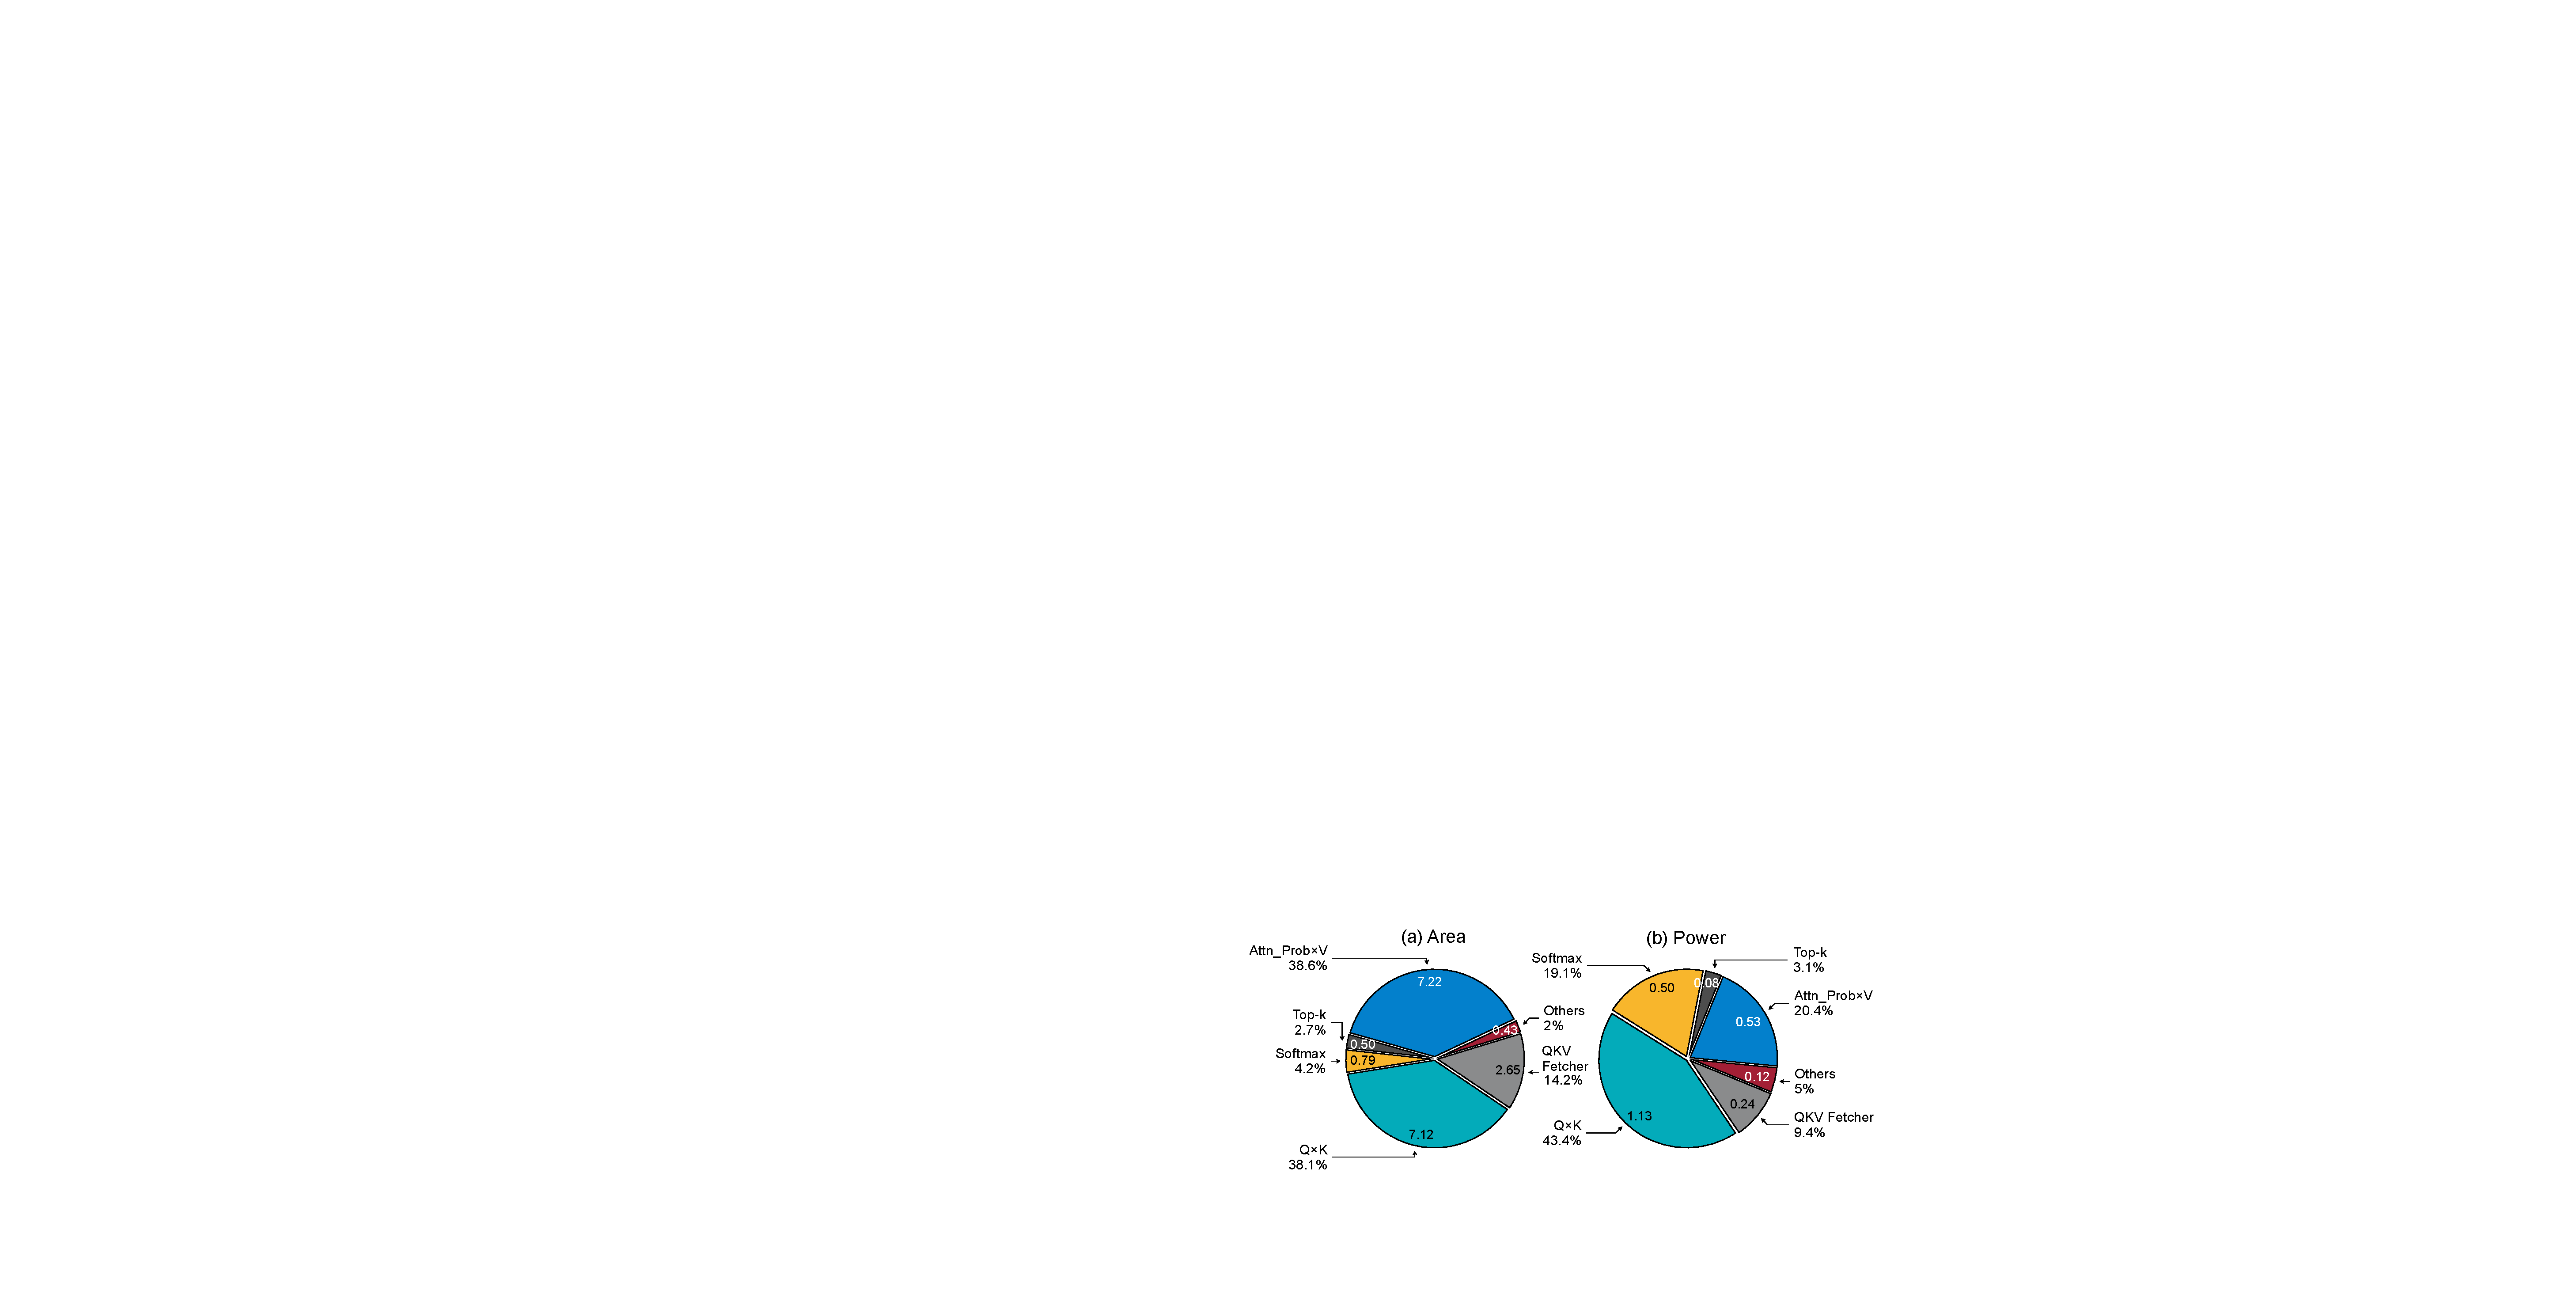
\includegraphics[width=1\columnwidth]{figures/pie.pdf}
    \caption{On-chip (a) Area and (b) Power Breakdowns of \spattenfull. 
    }
    \vspace{-15pt}
    \label{fig:pie}
\end{figure}
\begin{figure*}[t]
    \centering
    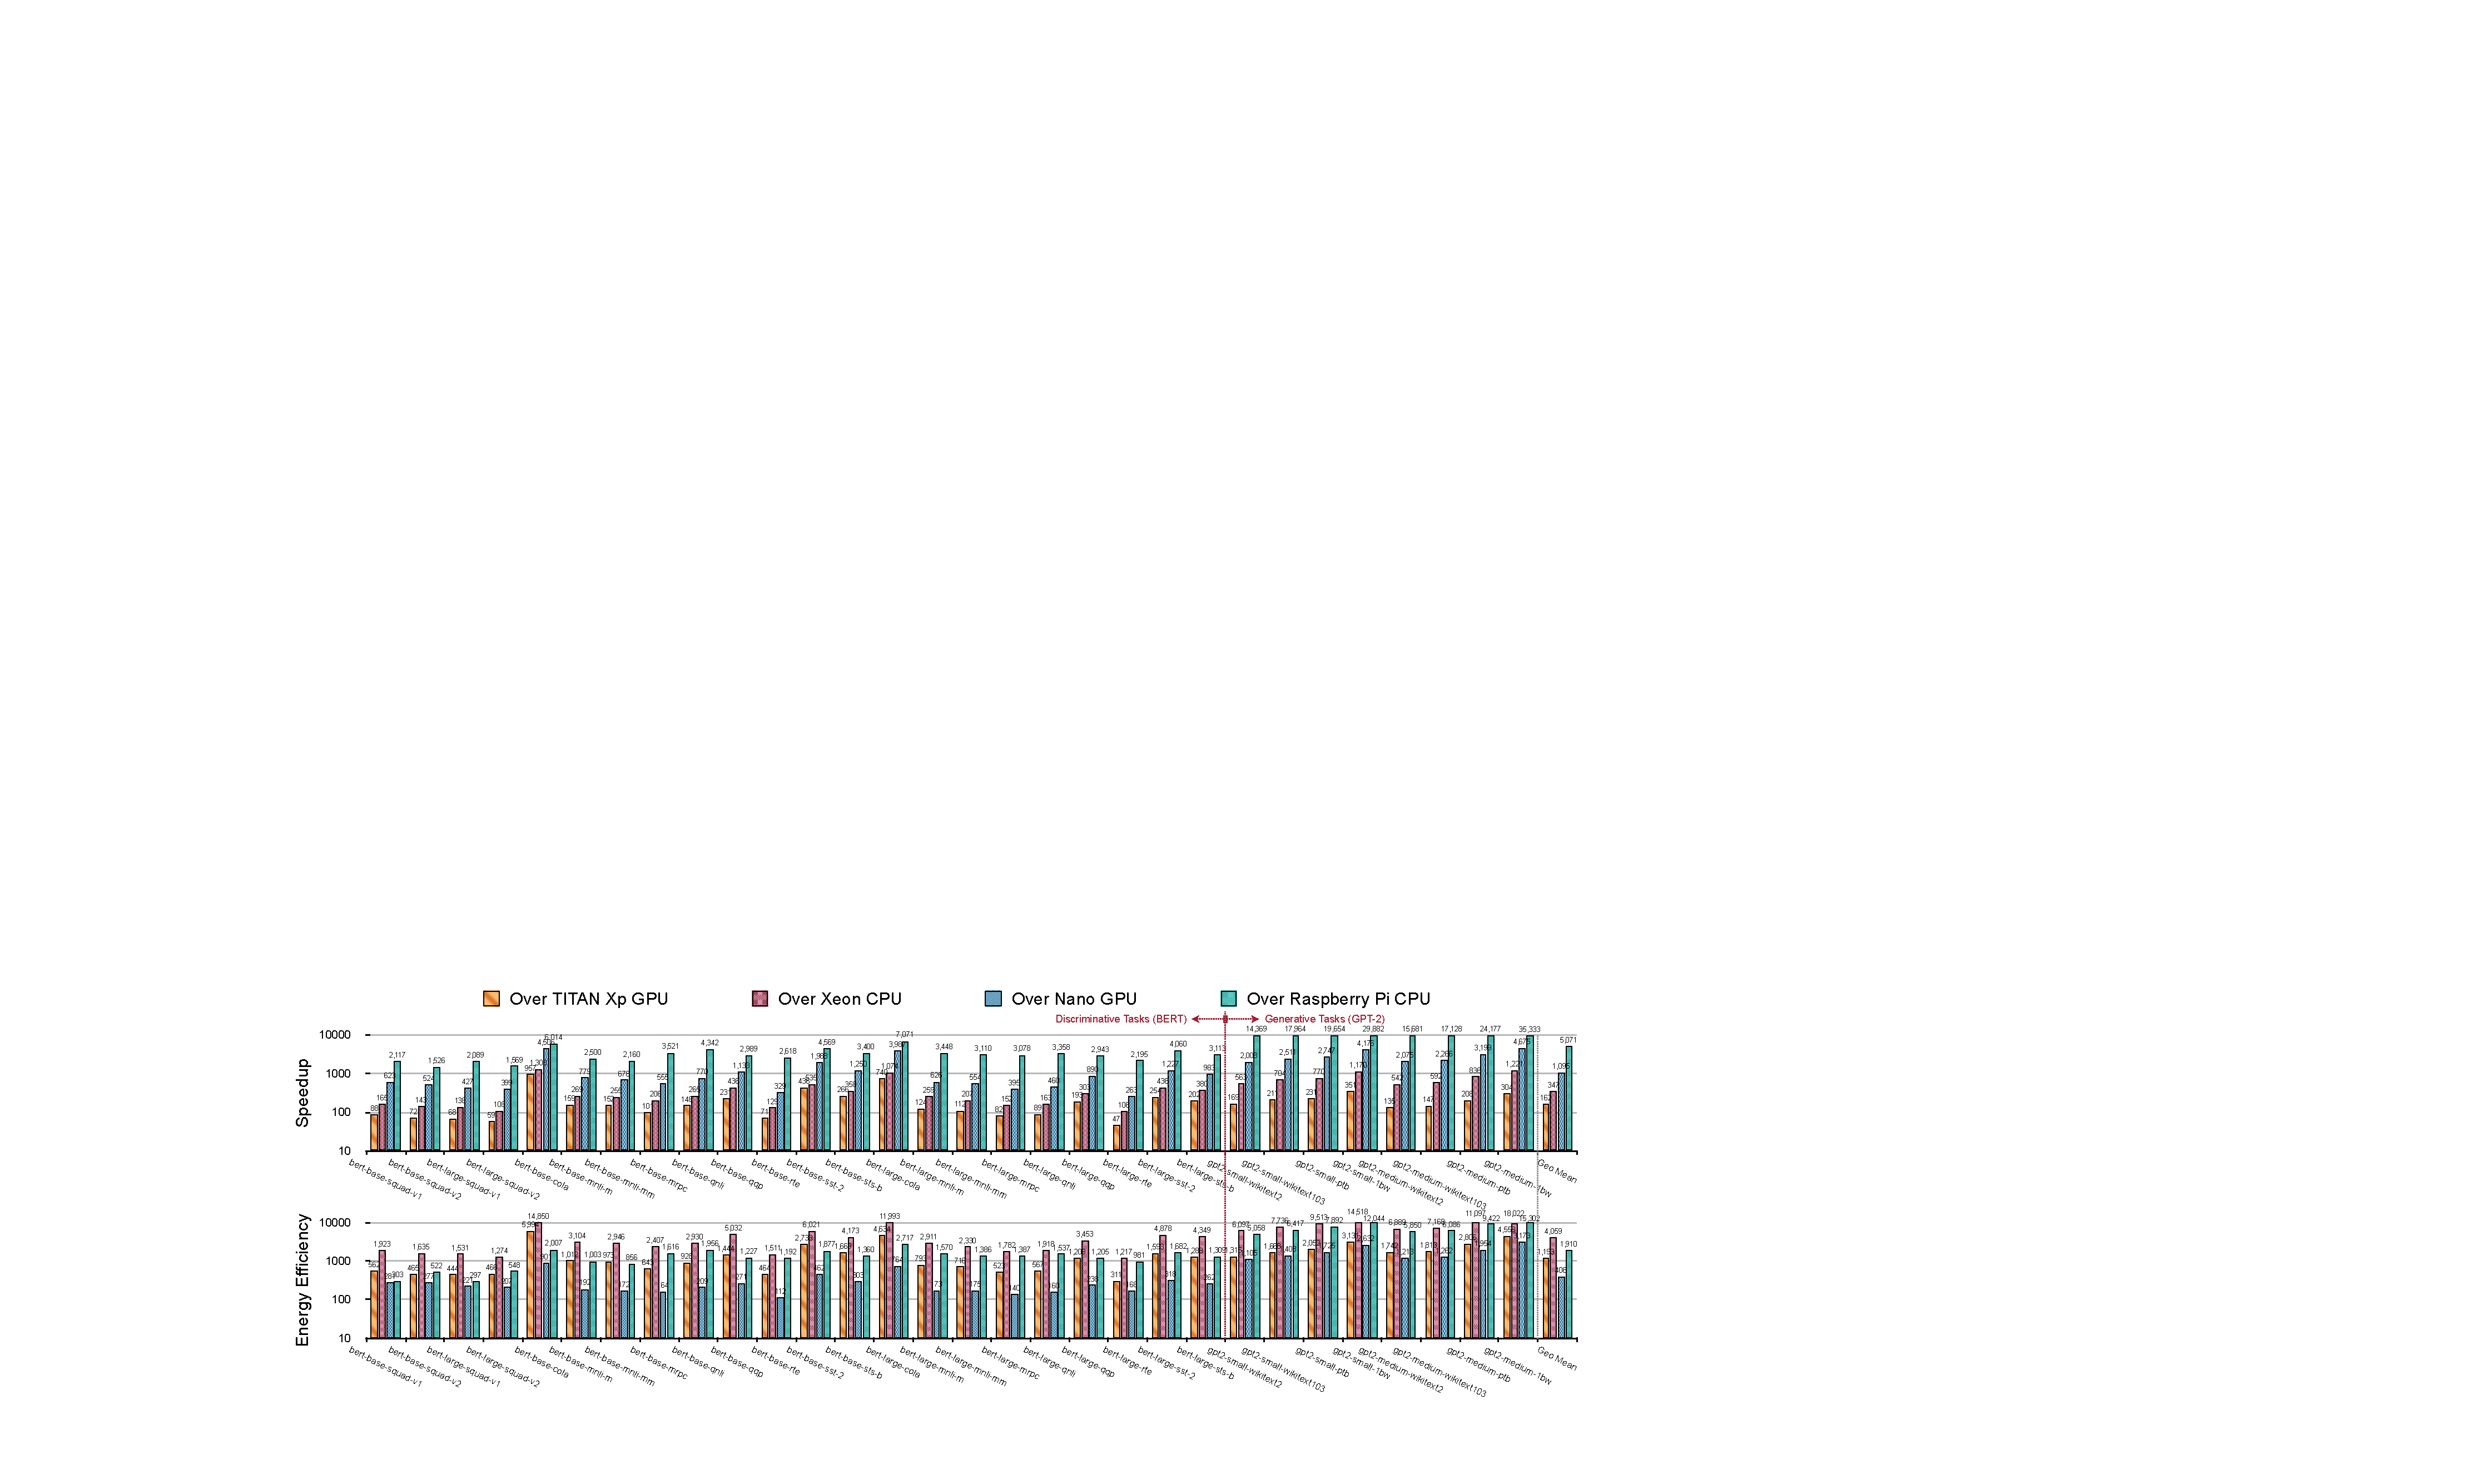
\includegraphics[width=1\textwidth]{figures/perfcomp.pdf}
    \vspace{-10pt}
    \caption{Speedup and Energy Efficiency of {\spattenfull} over baselines on attention layers. \name can accelerate both discriminative and generative models. 
    }
    \vspace{-10pt}
    \label{fig:perfcomp}
\end{figure*}


\textbf{Throughput, Power, and Area.}
\name prunes tokens and value vectors with cascade token pruning and local value pruning by \prunedramsaving\x (all models average), and \prunegpttwodramsaving\x (\gpttwo models average). Cascade head pruning has \hpdramsaving\x reduction on average. Note that the pruning ratio can be larger when the input sentence of a task is longer because they contain more redundancy. GPT-2 models have longer inputs than BERT, so their pruning ratios can be larger.
\name reduces the computation by \totalcompsaving\x and DRAM access by \totaldramsaving\x on average. It achieves \spattenbertflops\tflopss on 22 computation-bounded \bert models and \spattengpttwoflops\tflopss on 8 memory-bounded \gpttwo models. {\spattenfull} consumes \powerspattenfull W power as in Table~\ref{tab:powerbreak} breakdown and is \areaspattenfull mm$^2$ in area. 
Figure~\ref{fig:pie} shows the area and on-chip power breakdown. 
The Q$\times$K and Attention\_Prob $\times$V modules consume largest portions of energy and area since they are two most computational intensive modules. The latter consumes less energy thanks to local V pruning. \topk engines are relatively efficient, only taking \topkpowerratio\xspace of overall power and \topkarearatio\xspace of area so will not cause severe congestion issues.


\textbf{Comparisons with CPUs and GPUs.}
Figure~\ref{fig:perfcomp} shows the speedup and energy efficiency comparisons of \spattenfull\xspace with baselines on attention layers of the benchmarks. 
On average, \name achieves \perfovertitanxp\x, \perfoverxeon\x, \perfovernano\x, and \perfoverrasp\x speedup, and \eeovertitanxp\x, \eeoverxeon\x, \eeovernano\x, and \eeoverrasp\x energy saving over \titanxp, \xeon, \nano, and \rasp.
\name obtains high speedup because it has a highly parallelized and pipelined datapath. Meanwhile, cascade pruning and progressive \lowprec further reduce computation and DRAM access. Energy savings mainly come from DRAM fetch reduction. The specialized datapath also reduces intermediate SRAM fetch. 
Since FFN layer computations are reduced by token pruning, CPUs and GPUs can also be accelerated. 
We implement token pruning on CPUs/GPUs. We use \texttt{topk} and \texttt{gather} operations to select un-pruned tokens and QKV matrices to reduce matrix sizes, thus reducing computation, latency, and memory footprint. 3\x pruning ratio brings up to 2.3\x speedup for BERT in batch mode (assume performing token pruning twice). GPT-2 results in Figure~\ref{fig:perfcomp} do not have Beam Search. However, our techniques can also accelerate the Beam Search case because when a token (and its K, V) is pruned, it \emph{will not be used by any beams}.

\begin{table}[t]
\centering
\renewcommand*{\arraystretch}{0.1}
\setlength{\tabcolsep}{1pt}
\footnotesize
\centering
\caption{Compare \spattensmall with prior art \athree and \mnnfast.}
\vspace{-5pt}
\begin{tabular}{l|c|c|c}
\toprule
& \mnnfast & \athree & \textbf{\spattensmall}  \\
\midrule
\midrule
Cascade Head Pruning & \xmark & \xmark & \cmark \\
\midrule
Cascade Token Pruning & \xmark & \xmark & \cmark \\
\midrule
Interpretable Pruning & \xmark & \xmark & \cmark \\
\midrule
Local Value Pruning & \cmark & \cmark & \cmark \\
\midrule
Progressive Quantization & \xmark & \xmark & \cmark \\
\midrule
Preprocessing Overhead & \xmark & \cmark & \xmark \\
\midrule
Reduce Computation of & Attention only & Attention only & Attention and FFN \\
\midrule
Accelerate & \bert only & \bert only & \bert \& \gpttwo \\
\midrule
\midrule
Technology & FPGA (28nm) & ASIC (40nm) & ASIC (40nm)  \\
\midrule
Frequency & 1GHz (projected) & 1GHz & 1GHz \\
\midrule
Area (mm$^2$) & - & 2.08 mm$^2$ & 1.55 mm$^2$  \\
\midrule
Throughput (GOP/s) & 120 (1\x) & 221 (1.8\x) & 360 (\perfovermnnfast\x) \\
\midrule
Energy Effi. (GOP/j)
 & 120 (1$\times$) & 269 (2.2$\times$) & 382 (\eeovermnnfast$\times$) \\
\midrule
Area Effi. (GOP/s/mm$^2$)
& - & 106 (1$\times$) & 238 (2.2$\times$) \\
\bottomrule
\end{tabular}
\label{tab:compa3}
\vspace{-20pt}
\end{table}


\textbf{Comparisons with \athree and \mnnfast.}
\athree~\cite{ham20203} and \mnnfast~\cite{8980322} are also attention accelerators exploring sparsity. \athree first sorts each dimension of the key vectors among all keys. Then it uses a pre-specified number of largest/smallest elements in the keys to conduct multiplications with a query and get \emph{partial} attention scores. If a score is smaller than a threshold, then the corresponding key will be pruned. \mnnfast removes V vectors whose attention probabilities are smaller than a threshold.
We compare the differences and performance of \spattensmall, \athree, and \mnnfast in Table~\ref{tab:compa3}. Specifically: (i) In \athree and \mnnfast, all QKV vectors need to be fetched from DRAM to on-chip buffers before determining what can be pruned, so it cannot reduce DRAM access. Thus, they can only accelerate computation-bounded models (discriminative \bert), but cannot accelerate memory-bounded models (generative \gpttwo). (ii) \athree has pre-processing overhead -- sorting the keys. (iii) Token pruning in \name is \emph{global and cascade}, while that in \athree is local in one head. Therefore, only \name can reduce the computation in both attention and FFN layers. (iv) Cascade token pruning is interpretable and can be intuitively visualized step by step (Figure \ref{fig:pruning_examples}). (v) \name also supports head pruning and progressive quantization.
\begin{figure}[t]
    \centering
    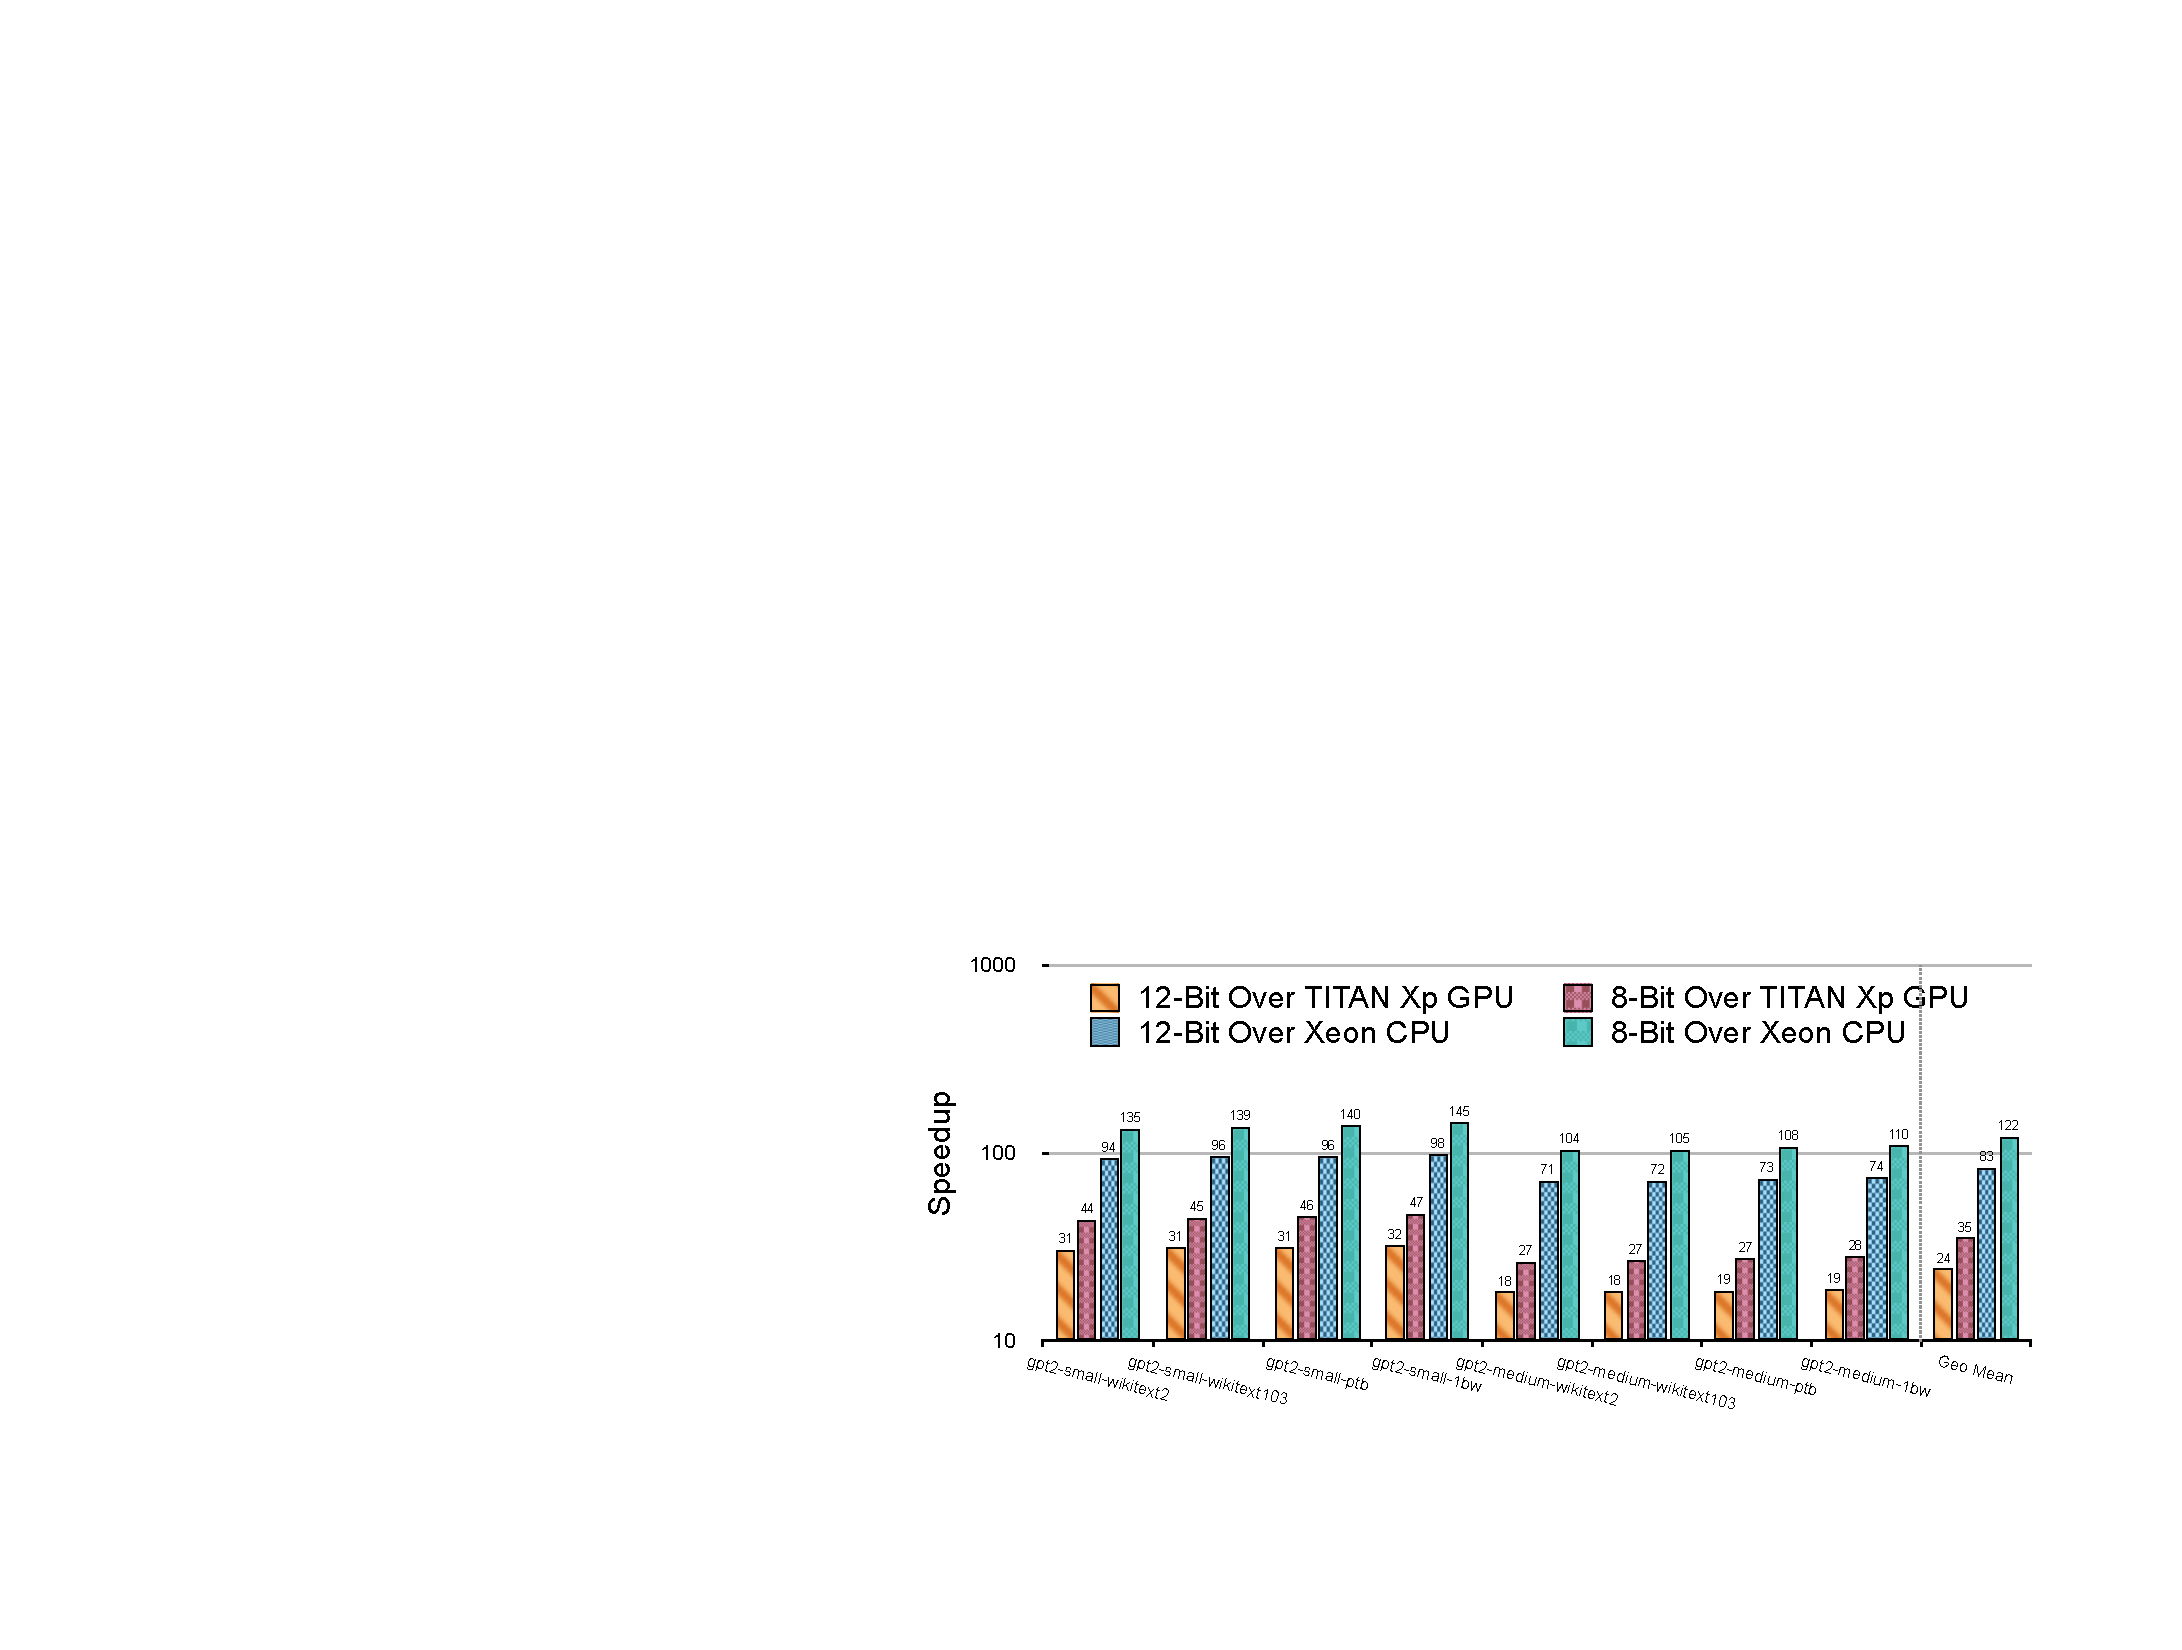
\includegraphics[width=1\columnwidth]{figures/perfcompfc.pdf}
    \vspace{-10pt}
    \caption{End-to-End speedup of {\spattenfc} over baselines. FC layer weights are quantized to 8 bits or 12 bits.}
    \vspace{-10pt}
    
    \label{fig:perfcompfc}
\end{figure}



\begin{table}[t]
\centering
\caption{FC \& Attention FLOPs \& Latency Breakdown on \gpttwo-Medium.}
\vspace{-5pt}
\setlength{\tabcolsep}{1pt}
\footnotesize
\centering
\begin{tabular}{l|c|c|c|c}
\toprule
& FC \gflops & Attn \gflops & FC Latency (ms) & Attn Latency (ms) \\
\midrule
GPU & 19.3 (85.6\%) & 3.3 (14.4\%) & 388.3 (51.4\%) & 366.7 (48.6\%) \\
\midrule
\textbf{\spattenfc} & 19.3 (95.5\%) & 0.9 (4.5\%) & 25.75 (92.4\%) & 2.13 (7.6\%)\\
\bottomrule

\end{tabular}
\label{tab:fc_attn}
\vspace{-10pt}
\end{table}


The parallelism $d$ in {\athree} is 64, corresponding to 128 multipliers. We compare \athree with {\spattensmall} which has the same number of multipliers (128), technology (40nm) and bandwidth (64GB/s) in Table~\ref{tab:compa3}.
Under 1GHz, \athree throughput is 2$\times d$=128\gflopss. Since it has 1.73\x geomean speedup, the effective throughput is 128$\times$1.72=221\gflopss. We include the same DRAM power for \athree and \spattensmall. \spattensmall\xspace achieves \perfoverathree\x better throughput, \eeoverathree\x better energy efficiency, and \aeoverathree\x better area efficiency over \athree.
\mnnfast essentially only supports local Value pruning. We get its throughput number with our reproduced simulator under the same bandwidth and number of multipliers. \mnnfast was originally a Zynq-7020 FPGA design (10W power). As an optimistic estimation, we assume ASIC implementation consumes 10\x less power, \ie 1W. Compared to \mnnfast, \spattensmall\xspace has \perfovermnnfast\x higher throughput, and \eeovermnnfast\x better energy efficiency. 



\begin{figure}[t]
    \centering
    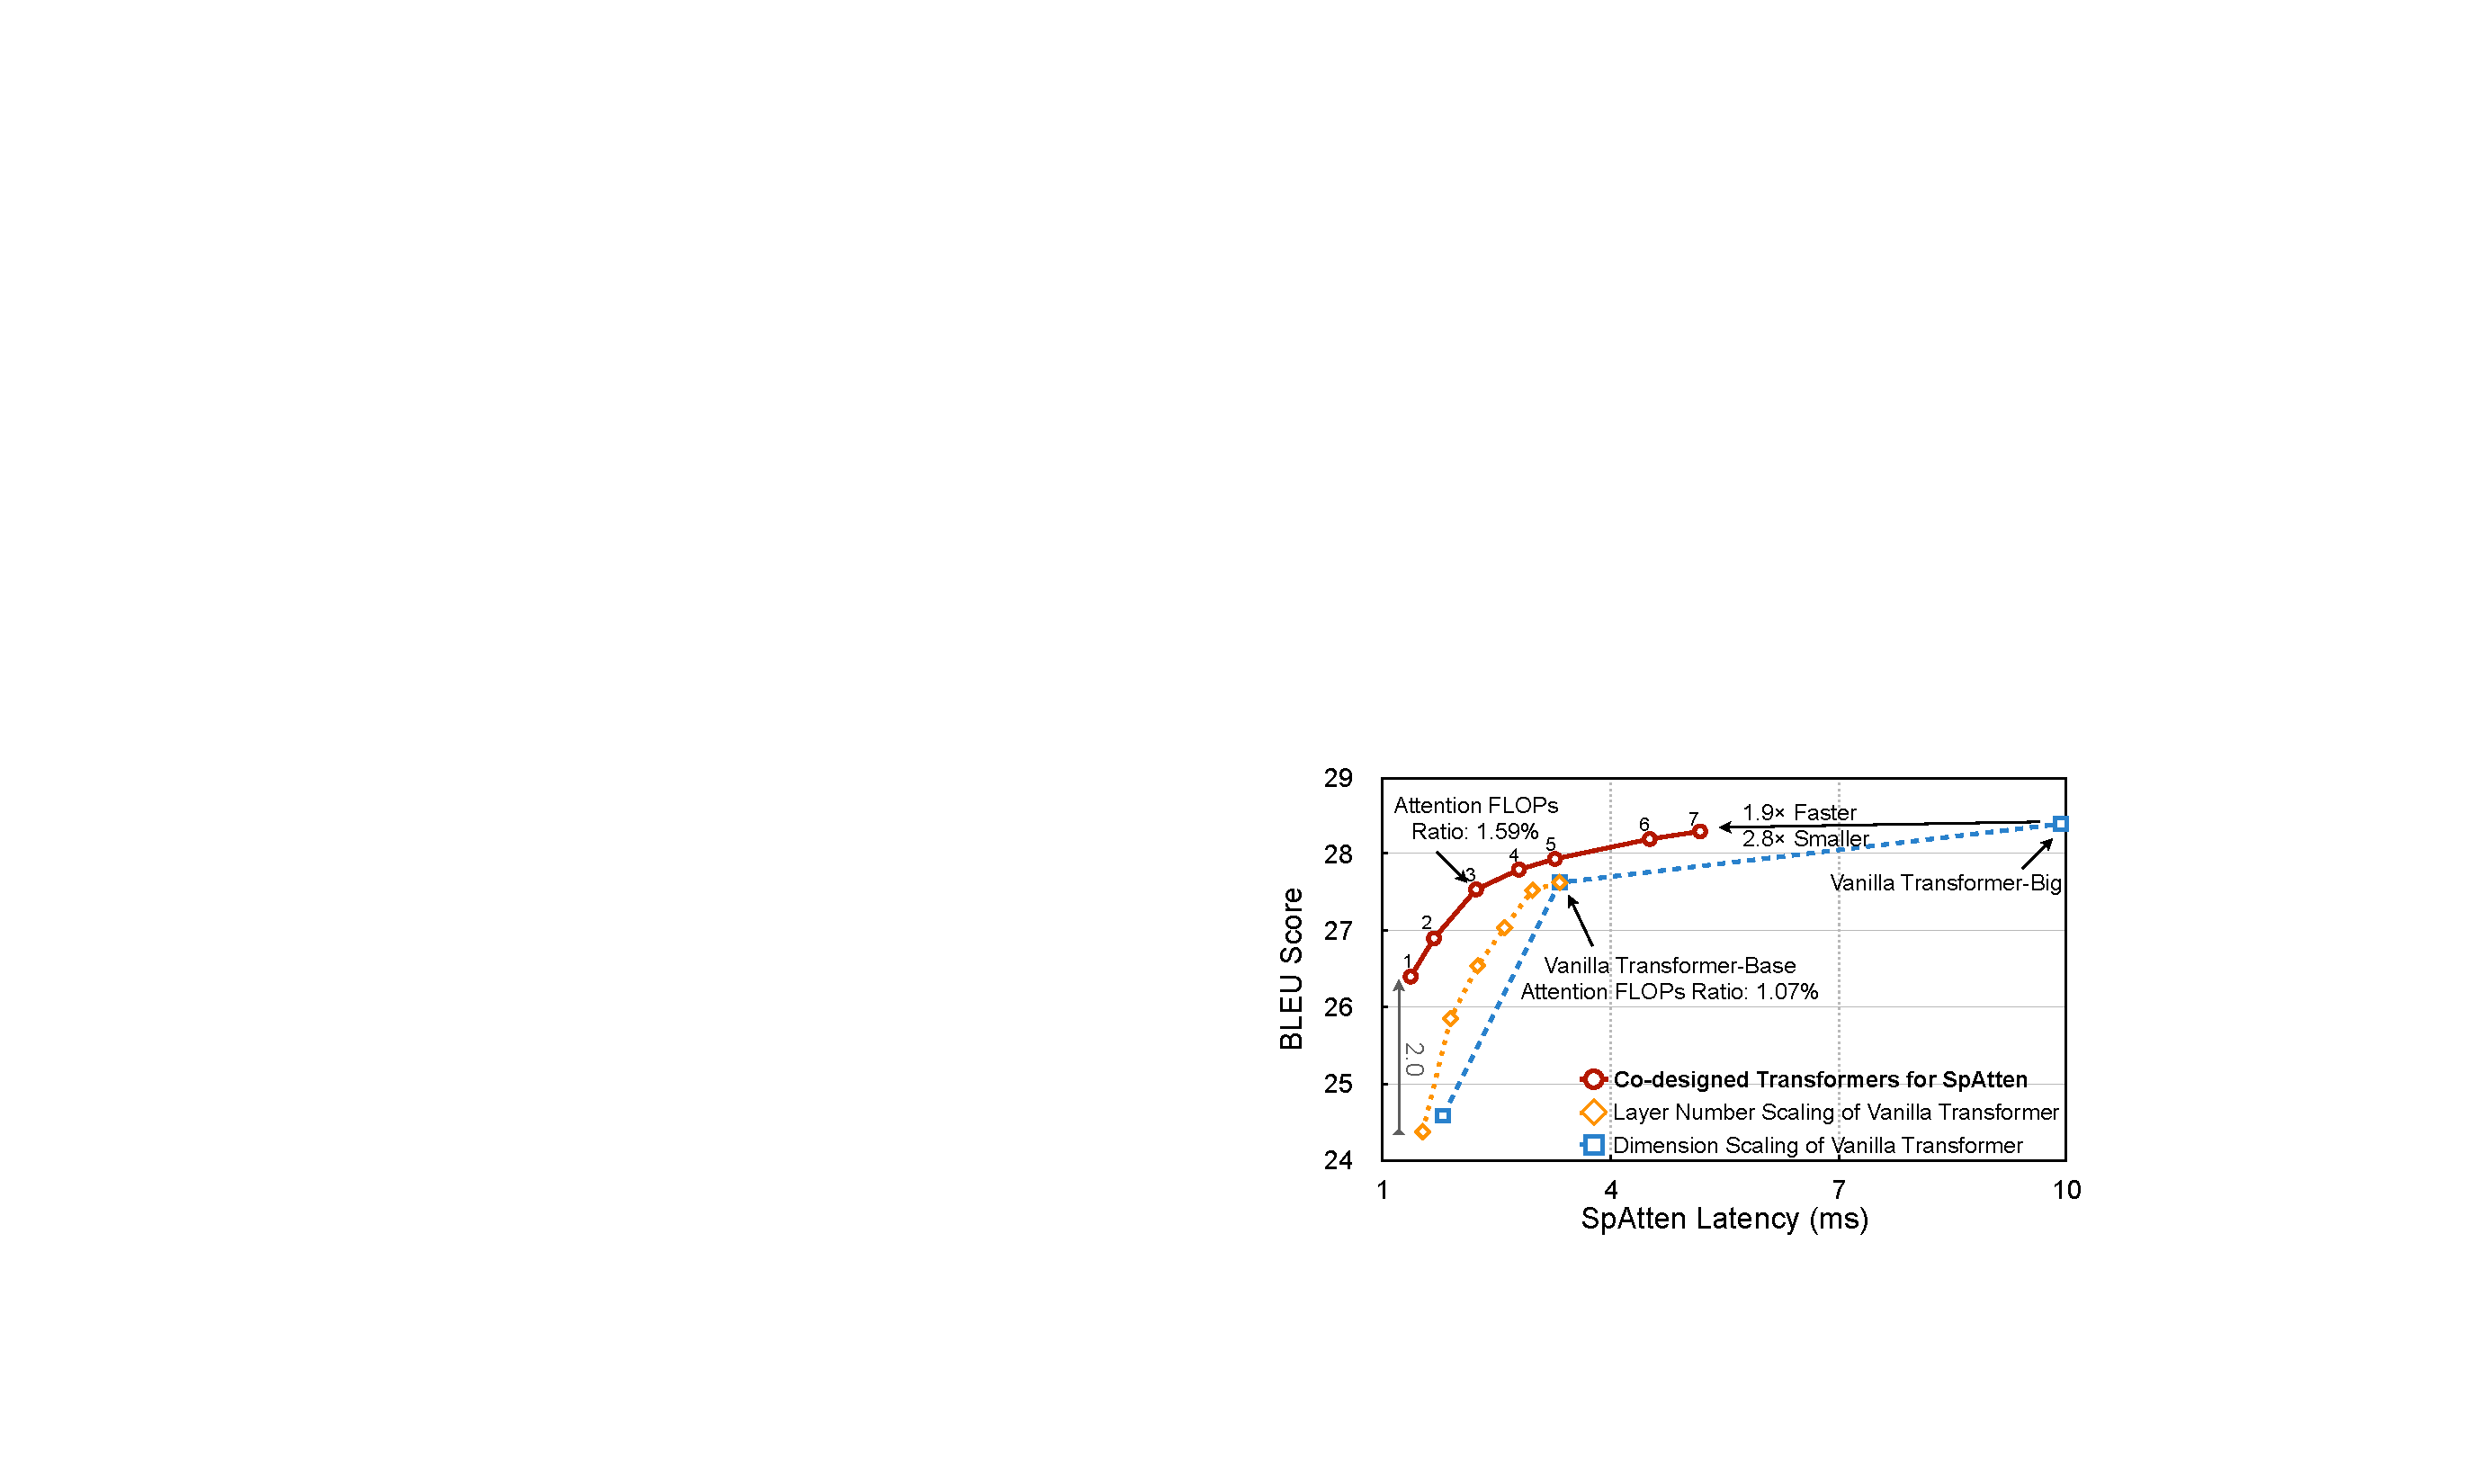
\includegraphics[width=\columnwidth]{figures/spattenhat.pdf}
    \vspace{-20pt}
    \caption{Co-designed Transformers for \spattenfc\xspace can achieve 1.9\x speedup and 2.8\x model size reduction over vanilla Transformers~\cite{46201}.
    }
    \label{fig:spattenhat}
    \vspace{-10pt}
\end{figure}


\textbf{End-to-End Performance with FFN Support.} To compare the end-to-end performance of \name with baselines. We extend our {\spattenfull} to support the FC in the  Feed-Forward Network (FFN) layers by reusing the multiplier arrays. The extended architecture is named {\spattenfc}.
FC weights are linear symmetrically quantized to 12 bits and 8 bits and stored on DRAM. Since the FCs in GPT-2 generation stage are matrix-vector multiplications, the performance of {\spattenfc} is memory-bounded. As shown in Figure~\ref{fig:perfcompfc}, on eight \gpttwo-Medium benchmarks, 8-bit FC \spattenfc\xspace achieves on-average \perffcovertitanxpteight\x and \perffcoverxeoneight\x speedup over \titanxp\xspace and \xeon; 12-bit FC \spattenfc\xspace achieves \perffcovertitanxptwelve\x and \perffcoverxeontwelve\x respectively. The breakdowns of computation and latency of FC and attention parts of four \gpttwo-Medium benchmarks averaged are shown in Table~\ref{tab:fc_attn}. Head pruning is not employed in this comparison. \spattenfc\xspace applies token pruning to reduce the attention FLOPs. The FC FLOPs are the same because token pruning can only reduce FC computation in the summarization stage (\bert), not the generation stage (\gpttwo). On GPU, the attention only accounts for 14.4\% computation but consumes 48.6\% latency, echoing with our analysis in Section~\ref{sec:motivation}. By contrast, attention on \spattenfc\xspace can be efficiently supported, thus only taking 7.6\% latency.

\textbf{Co-design Model Architecture with \name.} Besides the experiments above that leverage existing model architecture, we also explore the potentials of co-designing \name with model architecture by searching a 
Hardware-Aware Transformer (HAT)~\cite{hanruiwang2020hat} for \spattenfc. The search space contains [512, 640, 768] for embedding dim, [512, 1024, 2048, 3072] for FFN layer hidden dim, [1, 2, 3, 4, 5, 6] for decoder layer number, and last three layers for arbitrary encoder-decoder attention. Because the FC layers form the bottleneck of the \spattenfull\xspace performance, we intentionally configure the lower bound of FFN hidden dimension as low as 512 in expectation of reducing the FC ratio. We set different latency constraints and obtain a series of co-designed Transformers as shown in Figure~\ref{fig:spattenhat}. They are compared with layer number scaling and embedding dimension scaling of vanilla Transformer models~\cite{46201}. The co-designed Transformer-7 can achieve 1.9\x faster speed and 2.8\x smaller size over the vanilla Transformer-Big model. We also show the computation breakdowns of the vanilla Transformer-Base and the co-designed Transformer-3 in Figure~\ref{fig:barhat}. The two models have similar accuracy. Since \spattenfc\xspace can support attention with better efficiency, the co-designed model has a larger attention FLOPs. By virtue of the increased attention capacity, the FC computation can be largely shrunk without compromising the accuracy.



\subsection{Performance Analysis}
\textbf{Roofline Analysis.}
To better understand the distance of \spattenfull\xspace to the theoretical optimal performance, we analyze its roofline model in Figure~\ref{fig:roofline} and compare it with \titanxp. We use theoretical operational intensity: only memory access for input QKV and attention outputs are counted. HBM has 512GB/s bandwidth; thus, the slope of the bandwidth roof is 512G. \spattenfull\xspace has 1024 multipliers; hence the theoretical computation roof (multiplication and addition) is 2\tflopss. For \bert, the operation intensity is high, so the performance is computation-bounded. \spattenfull\xspace achieves \spattenbertflops TFLOPS on \bert tasks. That is close to the computation roof and higher than GPU's \gpubertflops\tflopss. \gpttwo models, on the contrary, have a low arithmetic intensity and appear in the memory-bounded region. \spattenfull\xspace achieves \spattengpttwoflops\tflopss, close to the bandwidth roof and higher than GPU's \gpugpttwoflops\tflopss. GPU performance is far from the roofs in both models because of the low utilization of computation units. Progressive \lowprec improves the computation intensity; thus, the points of \spattenfull\xspace are to the right of GPU.

\begin{figure}[t]
    \centering
    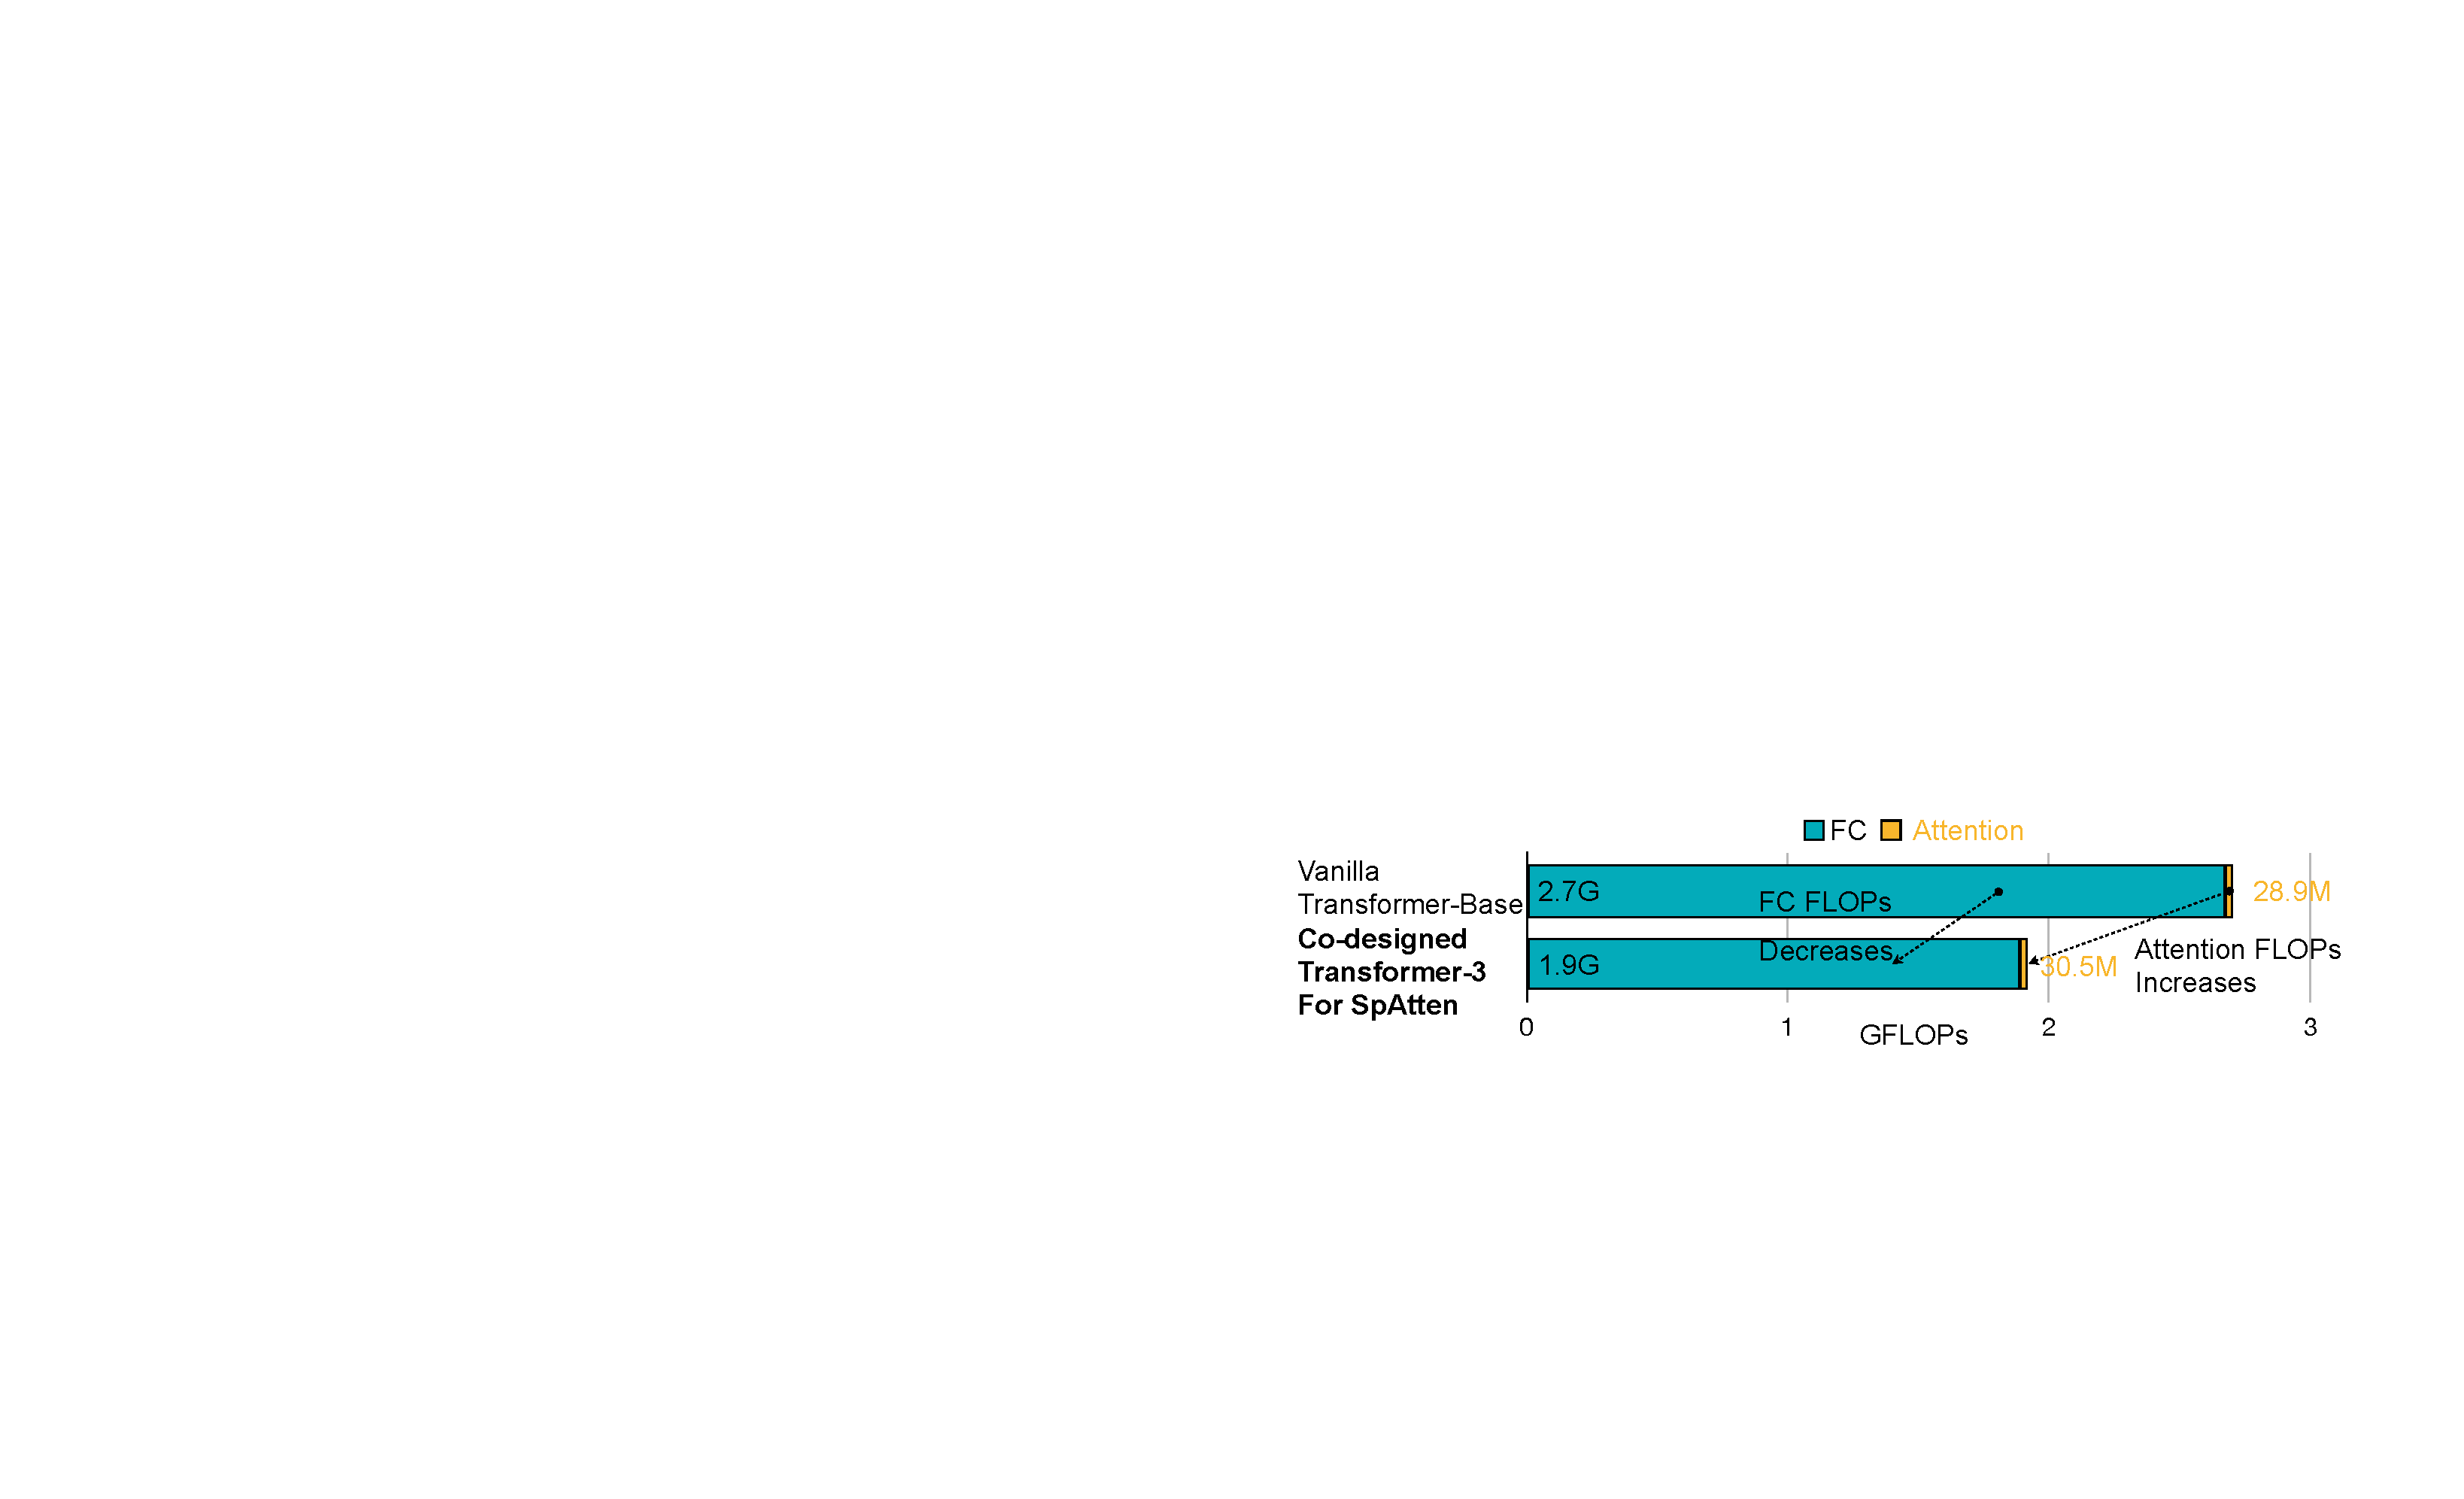
\includegraphics[width=\columnwidth]{figures/barhat.pdf}
    \vspace{-10pt}
    \caption{Co-designed Transformer has slightly more attention but much less FC computations because of \spattenfc's high efficiency on attention.
    }
    \label{fig:barhat}
    \vspace{-10pt}
\end{figure}

\textbf{Breakdown of Speedup.}
Figure~\ref{fig:perfbreak} shows the speedup breakdown of \spattenfull\xspace over \titanxp \xspace on eight \gpttwo benchmarks. With a dedicated datapath, \spattenfull\xspace is 22.1$\times$ faster than GPU baseline, which needs to execute numerous memory instructions for attention. Cascade pruning is then applied to remove unimportant tokens and heads in the second step, reducing computation by \prunegpttwodramsaving\x and \hpdramsaving\x, respectively. However, the performance only improves by 1.1$\times$ for both. The reason is that cascade pruning needs to frequently execute \topk to find unimportant tokens/heads, which becomes a bottleneck without a high throughput \topk engine. Therefore, after adding the high-parallelism \topk engine, the bottleneck is resolved, and the performance jumps by 3\x. Finally, the progressive \lowprec reduces the average \bitwidth of inputs, achieving another 2.8$\times$ speedup with less DRAM access.


\textbf{Efficiency-Accuracy Trade-offs.}
Without accuracy loss, token pruning can prune \prunedramsaving\x for all benchmarks on average, while head pruning can prune \hpdramsaving\x. Figure~\ref{fig:tradeoff} shows two trade-off curves between the token/head pruning ratio and accuracy of GPT-2-Small on PTB (left) and BERT-Base on CoLA (right). For the token pruning curve, head pruning is not applied, and vice versa. We apply 12-bit quantization and disable progressive quantization for both. We can prune around 4$\times$ tokens for PTB and 1.2$\times$ heads for CoLA without accuracy loss. Small pruning ratios even improve the accuracy. Note that the pruning ratio is related to the input sentence length. Since the sentence length of \gpttwo benchmarks (around 1000) is much longer than \bert ones (less than 100), \gpttwo's pruning ratios can be larger while preserving the accuracy.

\textbf{Design Choice Explorations.} We also explore the best architectural settings for \spattenfull\xspace in Figure~\ref{fig:ab2} on one \gpttwo application. The left side shows the performance with different parallelism (comparator number) of the \topk engine. 
Comparator number influences the time to perform a STATE\_RUN stage (see Algorithm~\ref{algorithm:topk}). 
After parallelism 16, the performance does not increase much because 16 matches the \topk engine input data rate from the Q$\times$K module. 
Thus parallelism larger than 16 makes \topk no longer the bottleneck and cannot much influence the overall performance. We select 16 in our design. 
On the right side, we change the size of SRAM storing K and V. Since \name supports up to 1024-length context, the minimum SRAM size is set to 2$\times$1024$\times$64$\times$12bits=196KB. `2' is for double buffering. Increasing SRAM size hardly increases the performance because the whole architecture is fully pipelined. More intermediate buffers will not significantly impact the throughput. 
Therefore, in consideration of reducing SRAM static power, we select the smallest 196KB.


\begin{figure}[t]
    \centering
    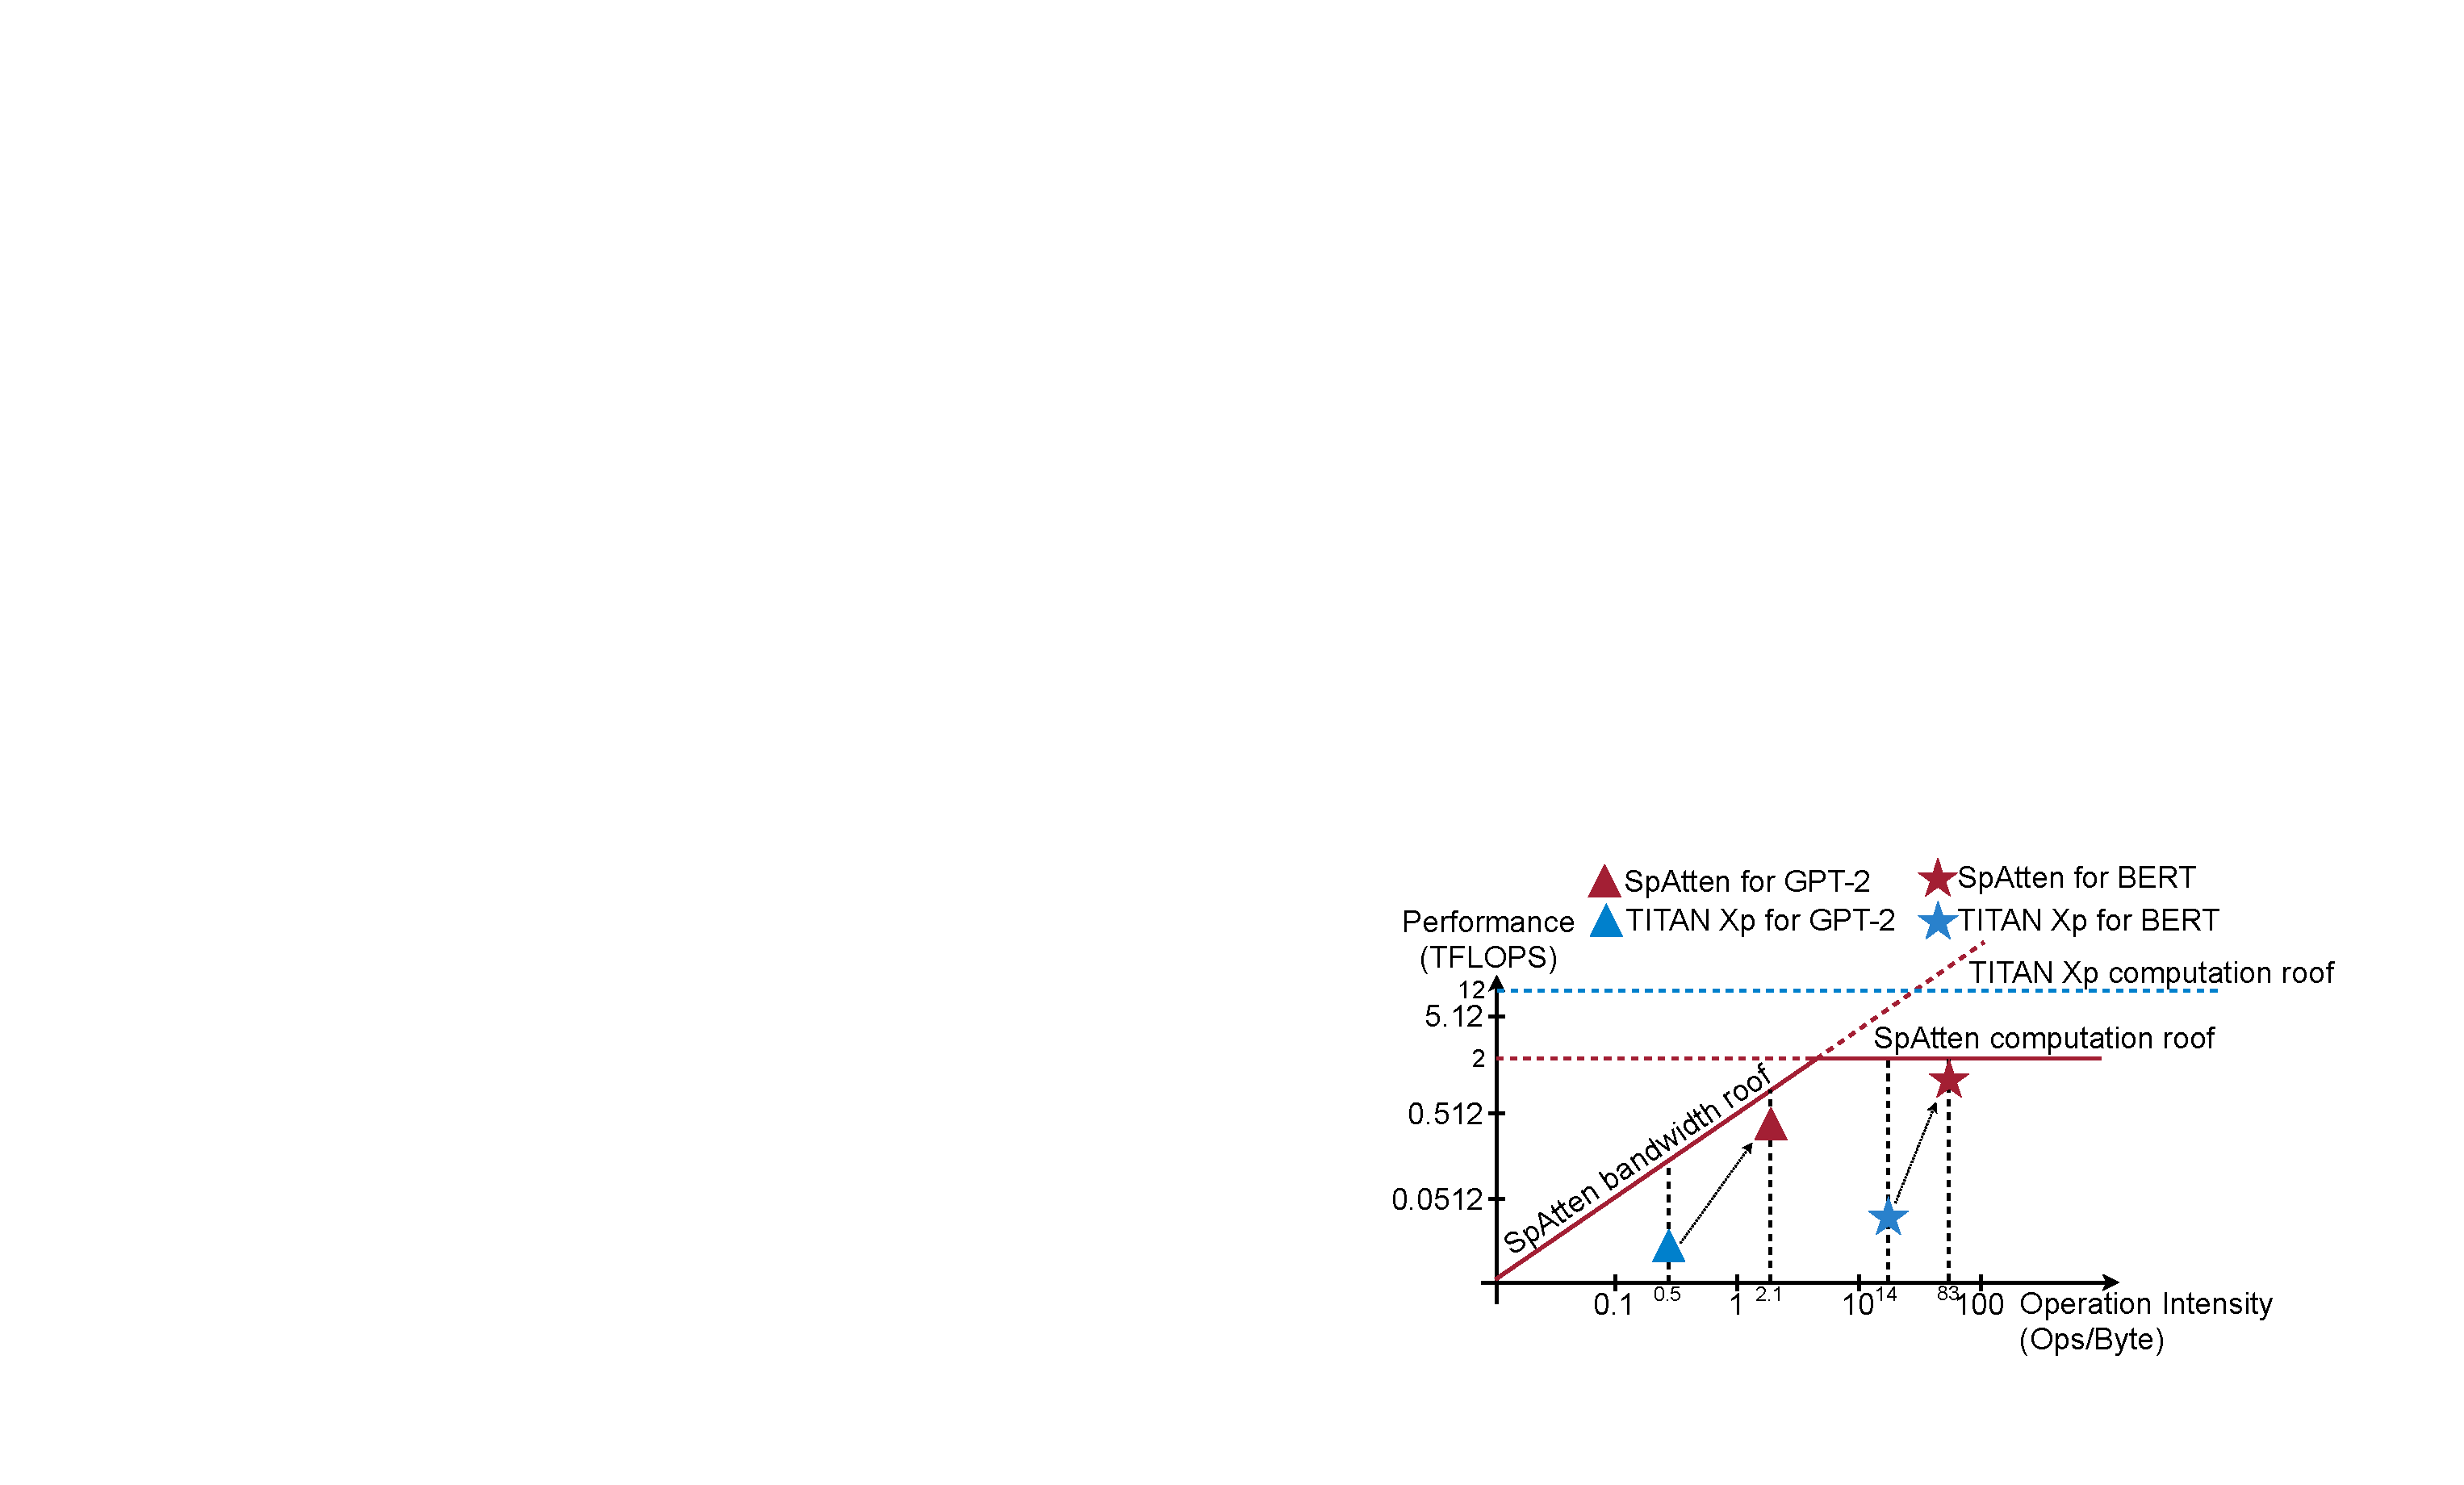
\includegraphics[width=\columnwidth]{figures/roofline.pdf}
    \vspace{-20pt}
    \caption{Roofline Model. The performance of \name is close to bandwidth and computation roofs.
    }
    \vspace{-15.5pt}
    \label{fig:roofline}
\end{figure}

\begin{figure}[t]
    \centering
    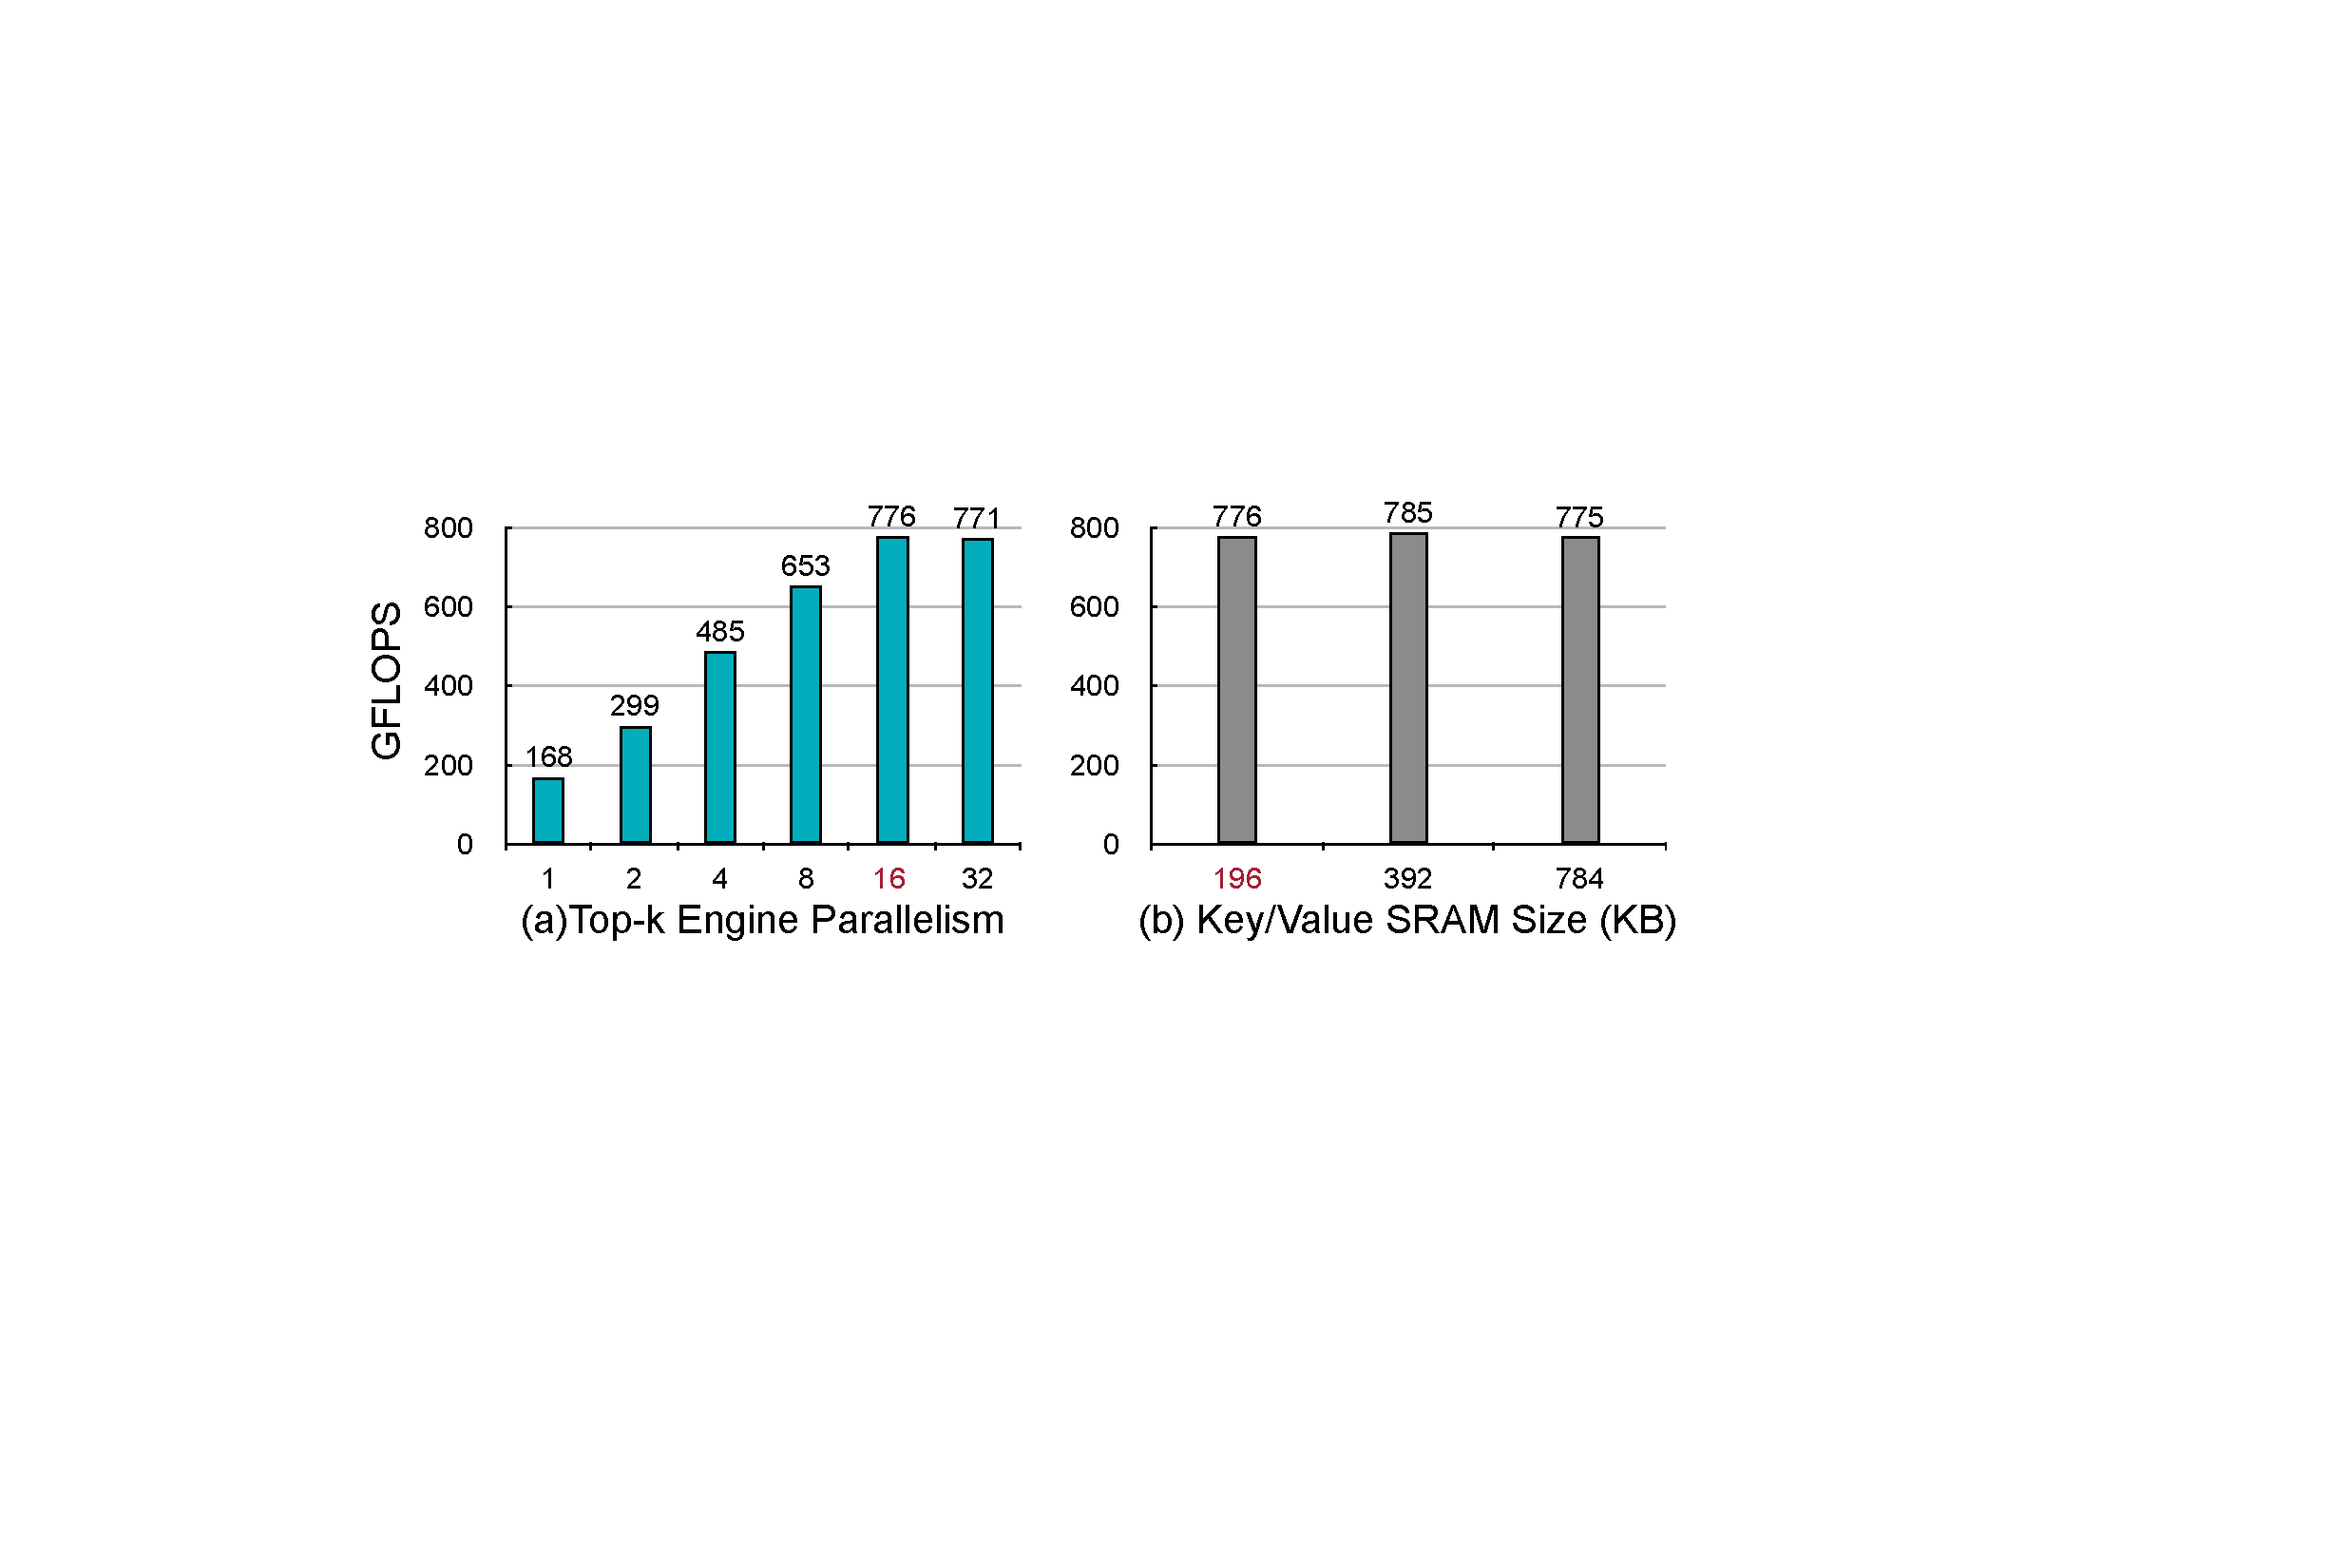
\includegraphics[width=\columnwidth]{figures/ab2.pdf}
    \vspace{-10pt}
    \caption{Design Space Exploration. A top-k engine with a parallelism of 16 and 196KB key/value buffer is sufficient for our settings.
    }
    \label{fig:ab2}
    \vspace{-10pt}
\end{figure}

\begin{figure}[t]
    \centering
    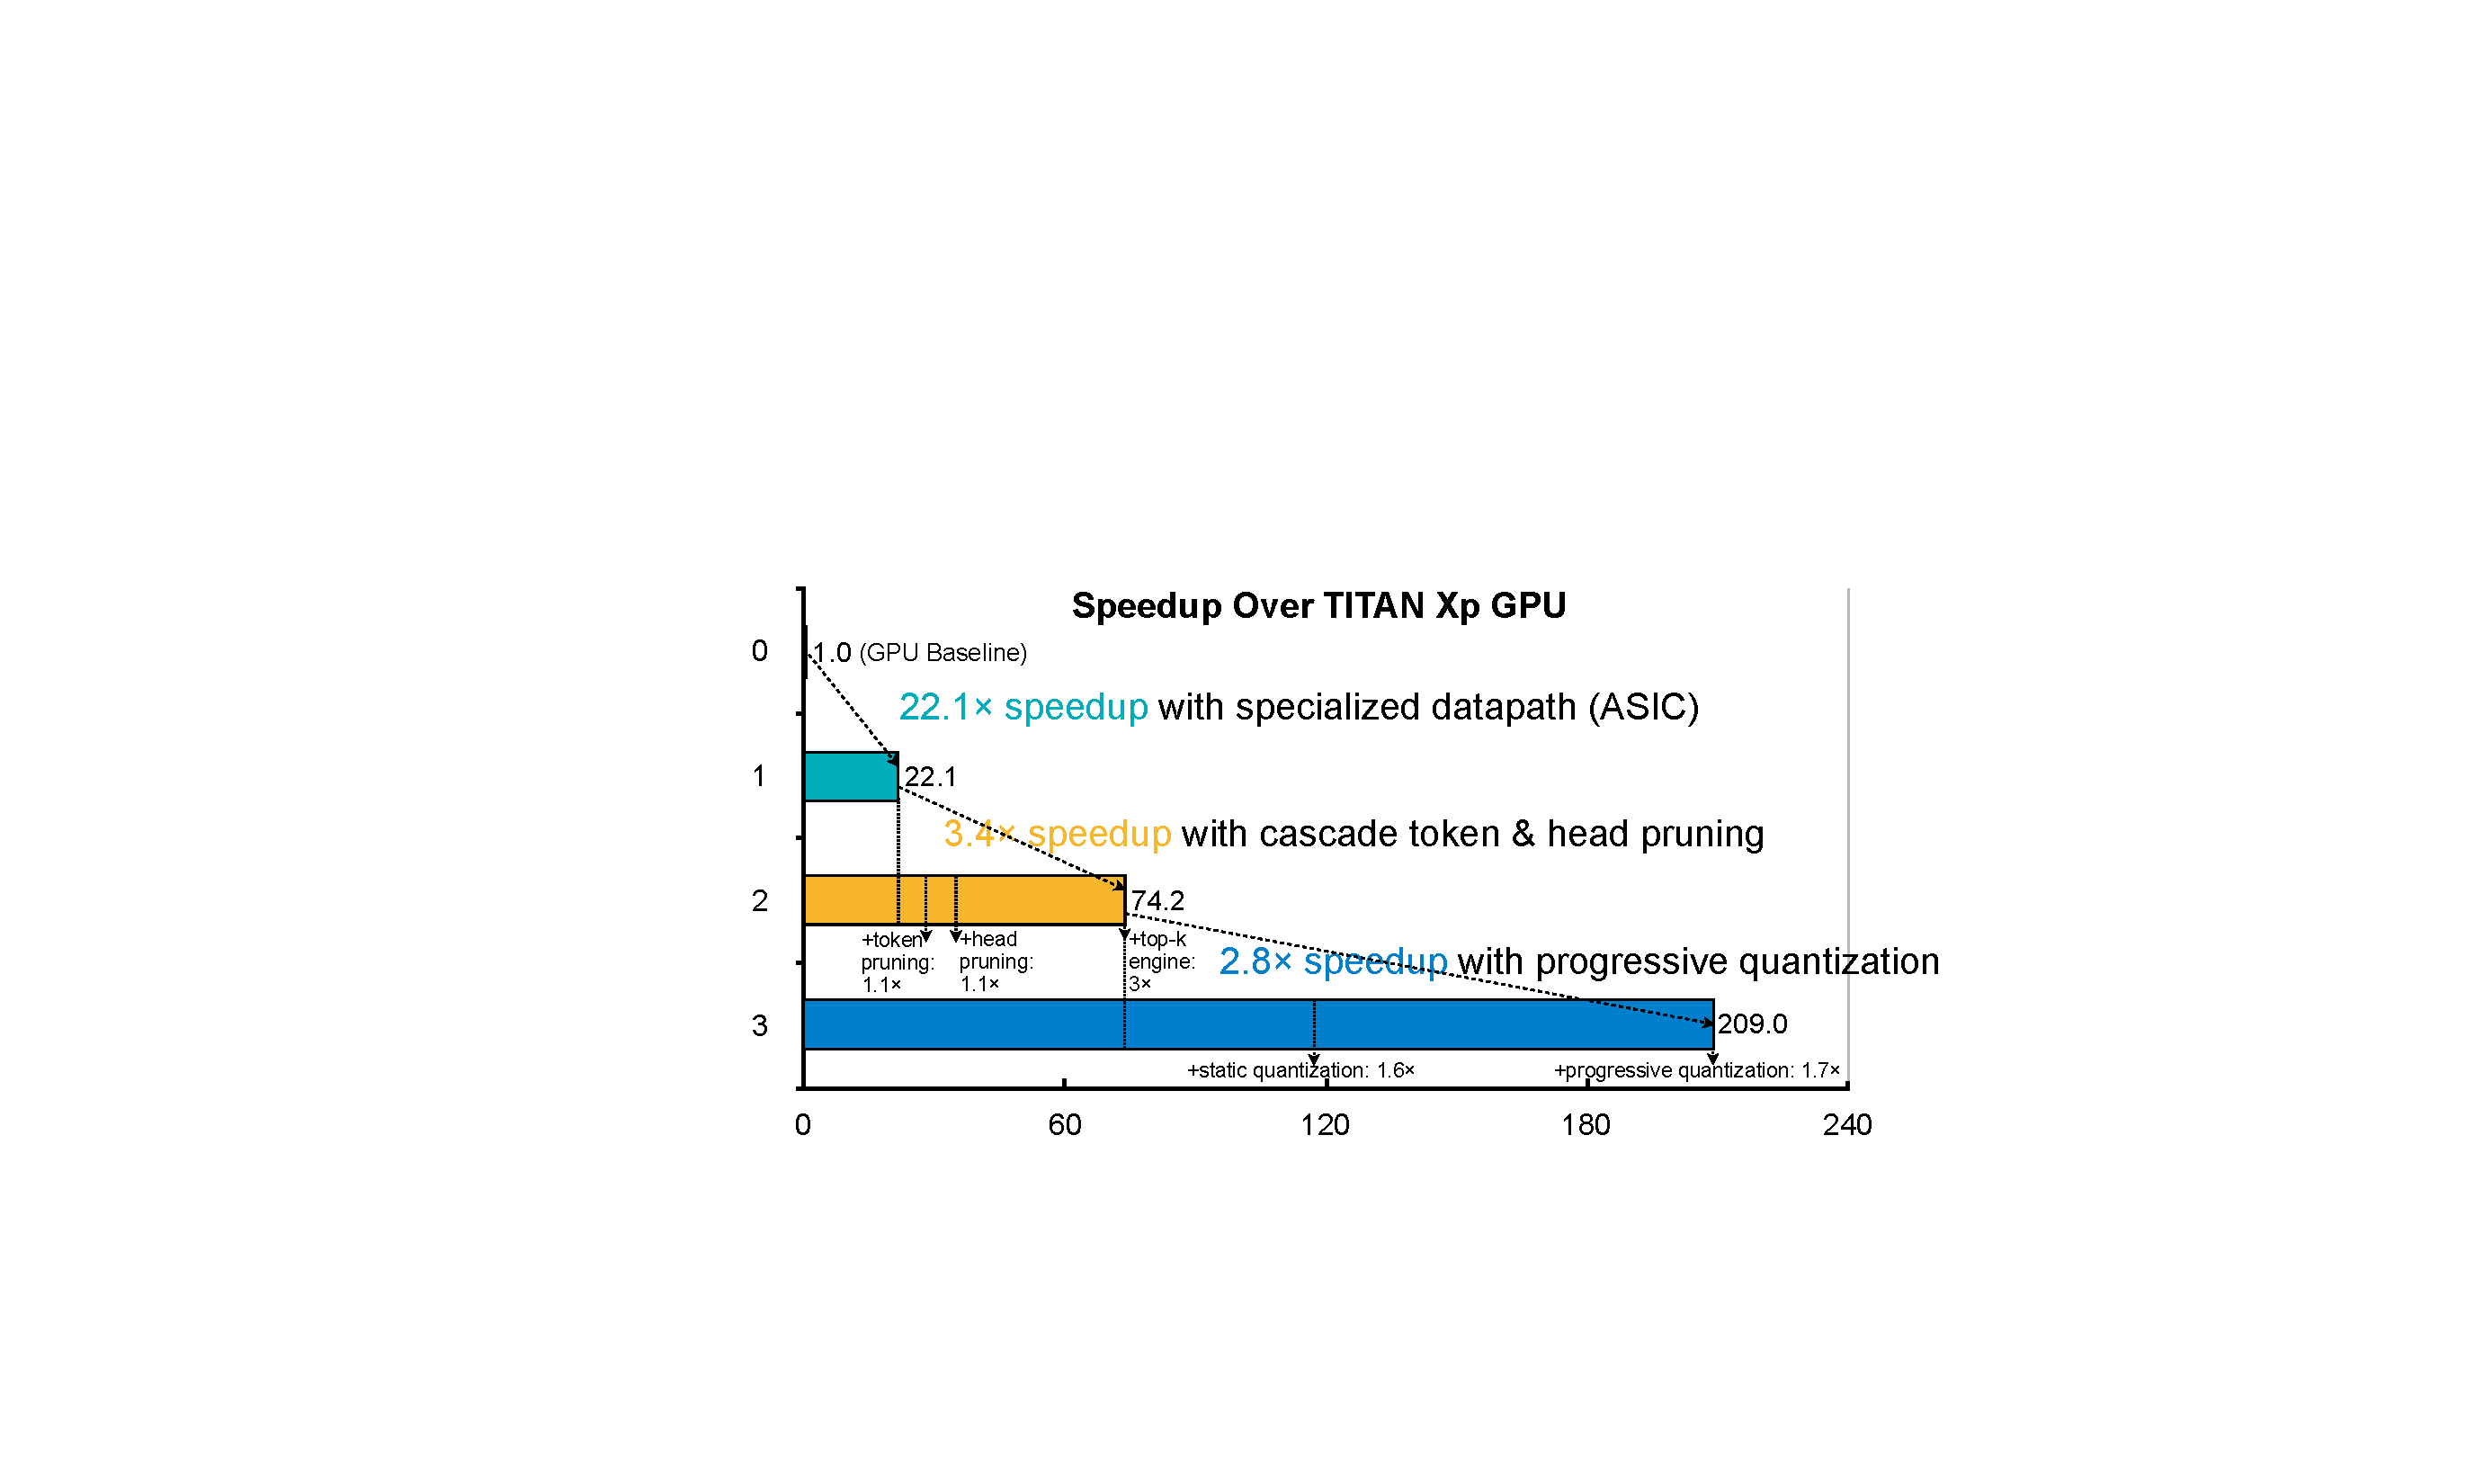
\includegraphics[width=\columnwidth]{figures/perfbreak.pdf}
     \vspace{-10pt}
    \caption{Speedup Breakdown of \name on \gpttwo models. Cascade pruning and progressive quantization bring 3.4\x and 2.8\x speedup, respectively.
    }
    \vspace{-5pt}
    
    \label{fig:perfbreak}
  
\end{figure}

\begin{figure}[t]
    \centering
    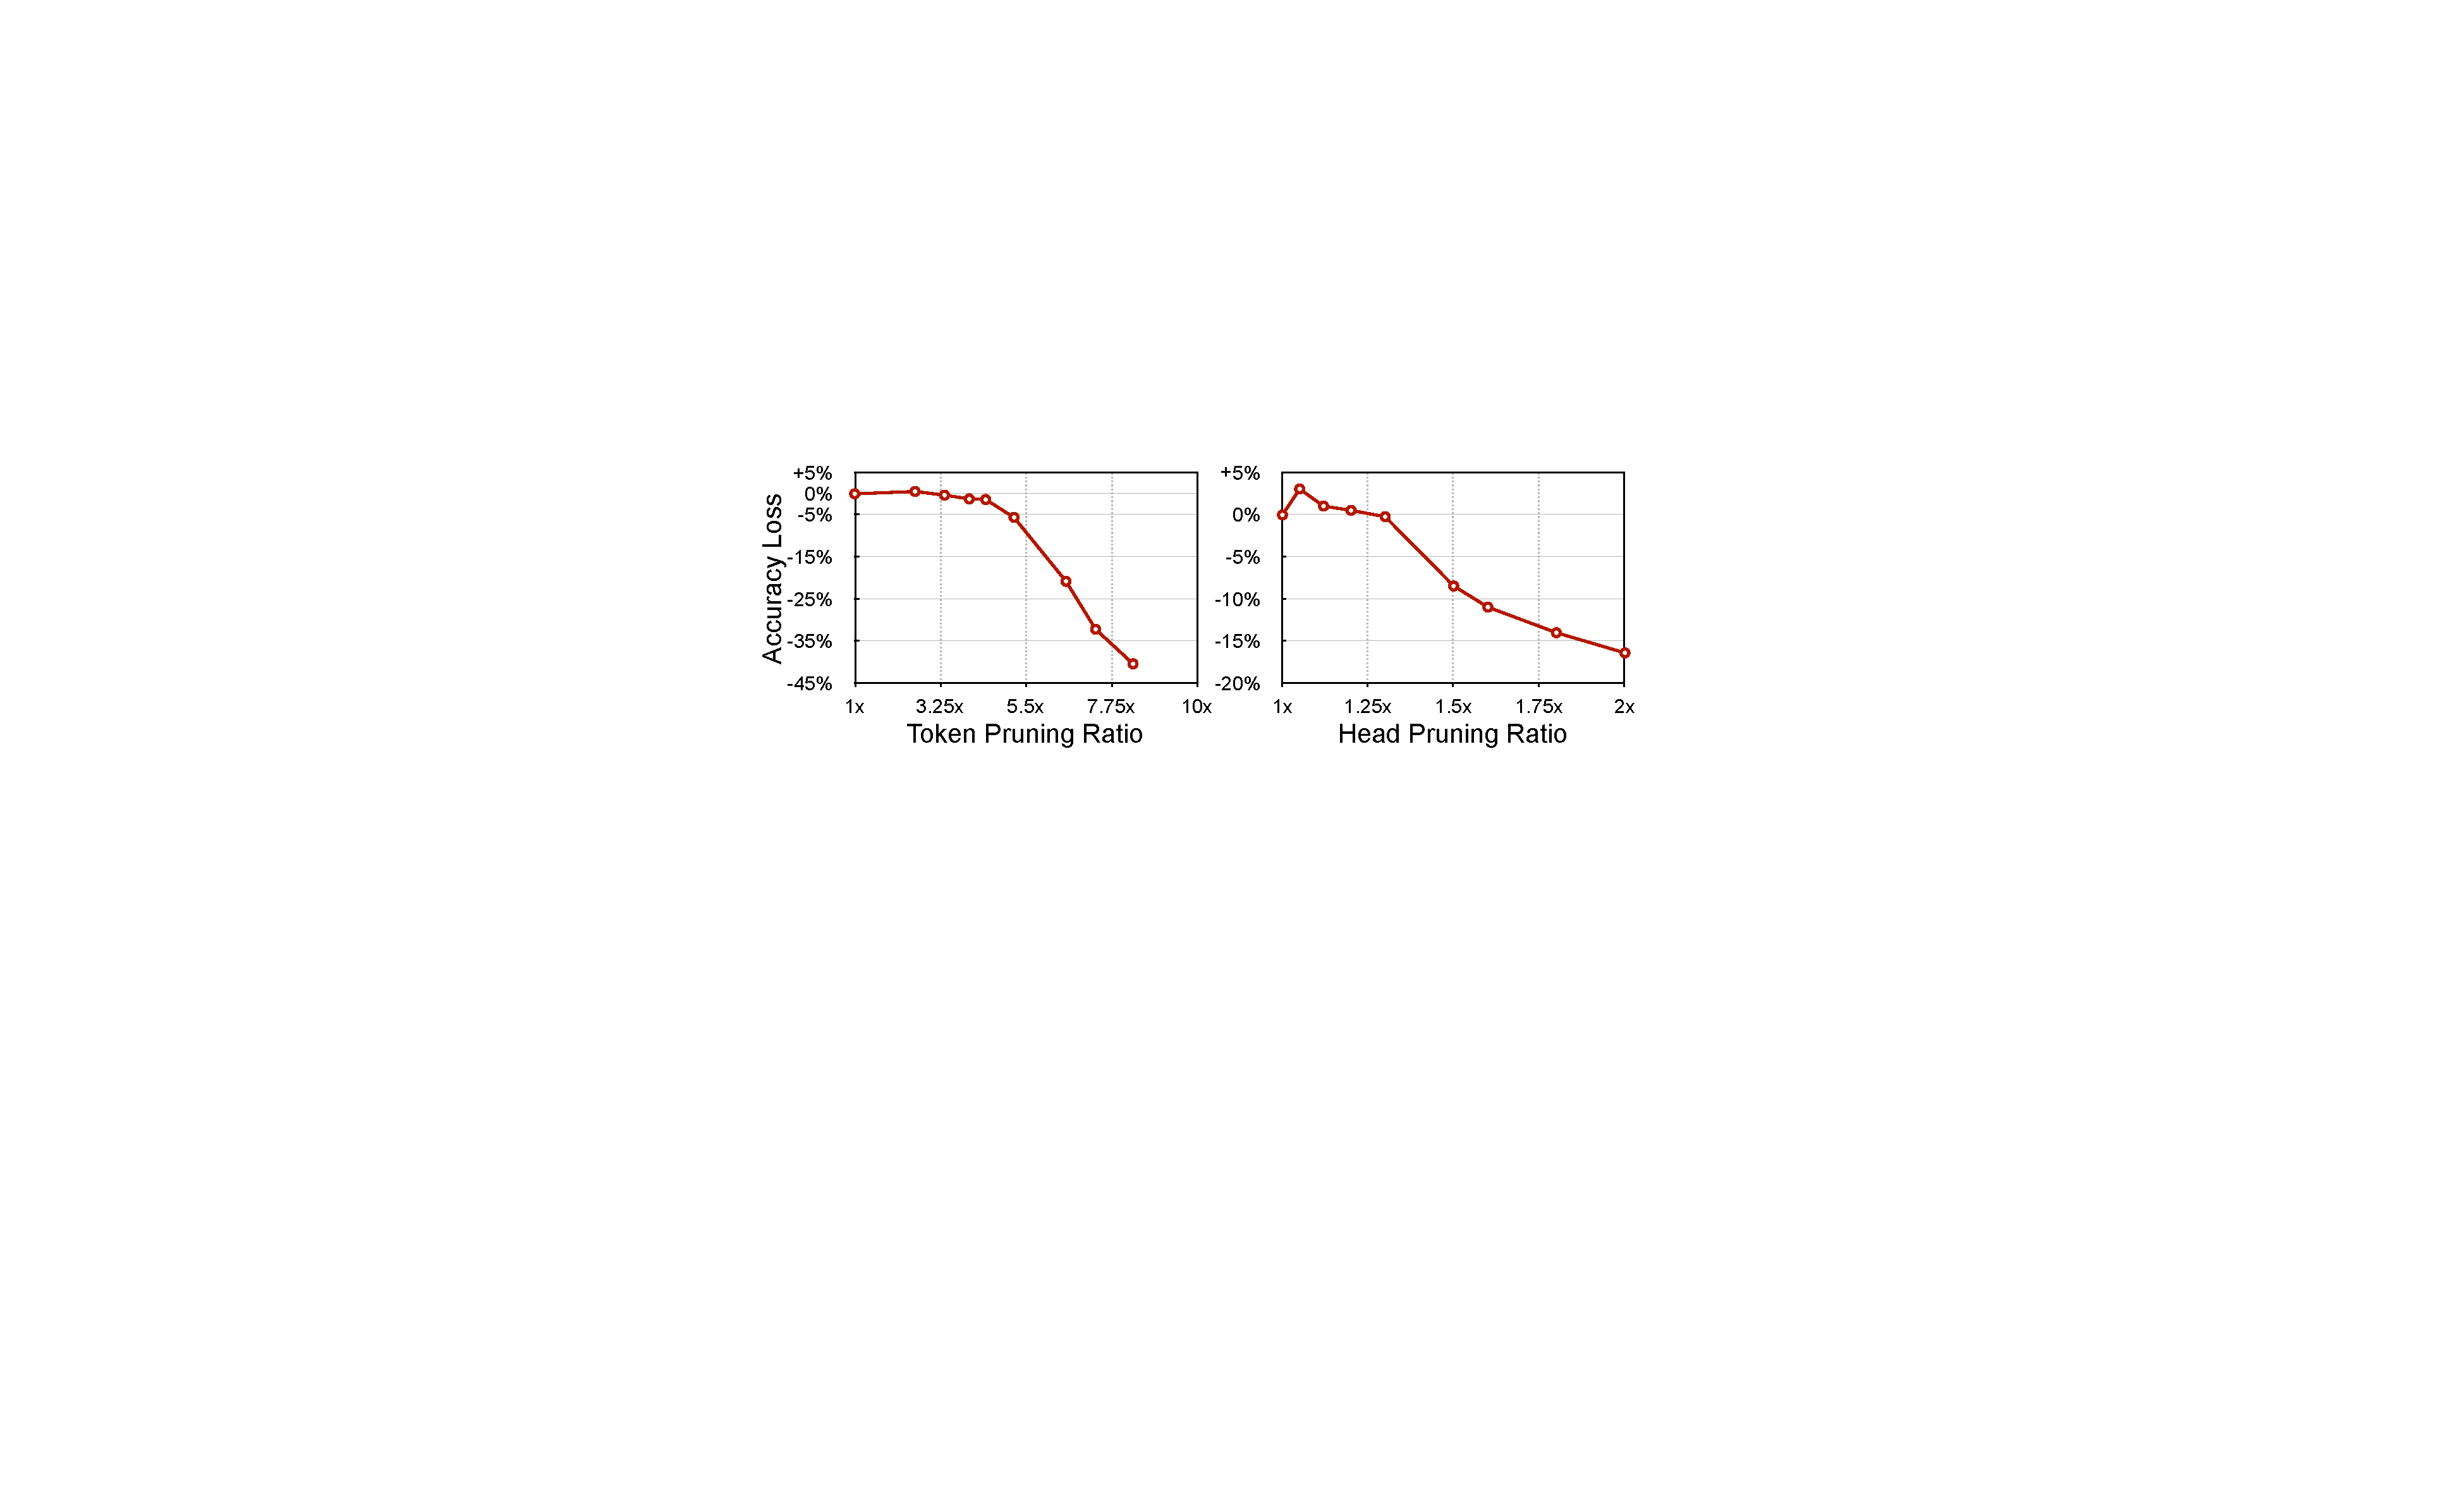
\includegraphics[width=\columnwidth]{figures/tradeoff.pdf}
    \vspace{-10pt}
    \caption{Trade-off curves between token/head pruning ratio and accuracy loss.}
    
    \label{fig:tradeoff}
    
    \vspace{-15pt}
\end{figure}


\textbf{Interpretation and Visualization.}
Figure~\ref{fig:pruning_examples} visualizes the cascade token pruning process on various tasks. The pruned tokens are redundant ones such as `it, are, to, is', showing the effectiveness of \name's importance score mechanism. 
In the first example, the tokens that survive pruning are `remember', `admire', `resolve confusion'; we can easily interpret why the sentence is classified as a positive sentiment.
The second example is the similarity score regression. The regressed scores range from 1 to 5, and larger scores indicate higher similarity between two sentences. \name can effectively prune away the meaningless tokens such as `your' and `is', and keep the token pairs in two sentences such as `upset' and `bothering'.
The last example is a generative language modeling with \gpttwo. The generated token is `English'. \name aggressively prunes away most tokens as they are irrelevant to the generated token, and only keeps `Du', `translate' and `into' tokens. The model may find the name `Du' not typical in English, so the translation language should be `English'.



Figure~\ref{fig:heatmap_gpt2} shows the cumulative importance scores of every single layer in a \gpttwo LM model. The important tokens are consistent across layers, such as `published'. Generated `papers' token heavily attends to several nearby tokens such as `published' and `many'. It also attends to some important tokens such as `researcher' and `architecture' even though they are far from it. In summary, token pruning reduces the model complexity and shows which tokens are attended most by the model, bringing better interpretability than \athree and \mnnfast.





\begin{figure*}[t]
    \centering
    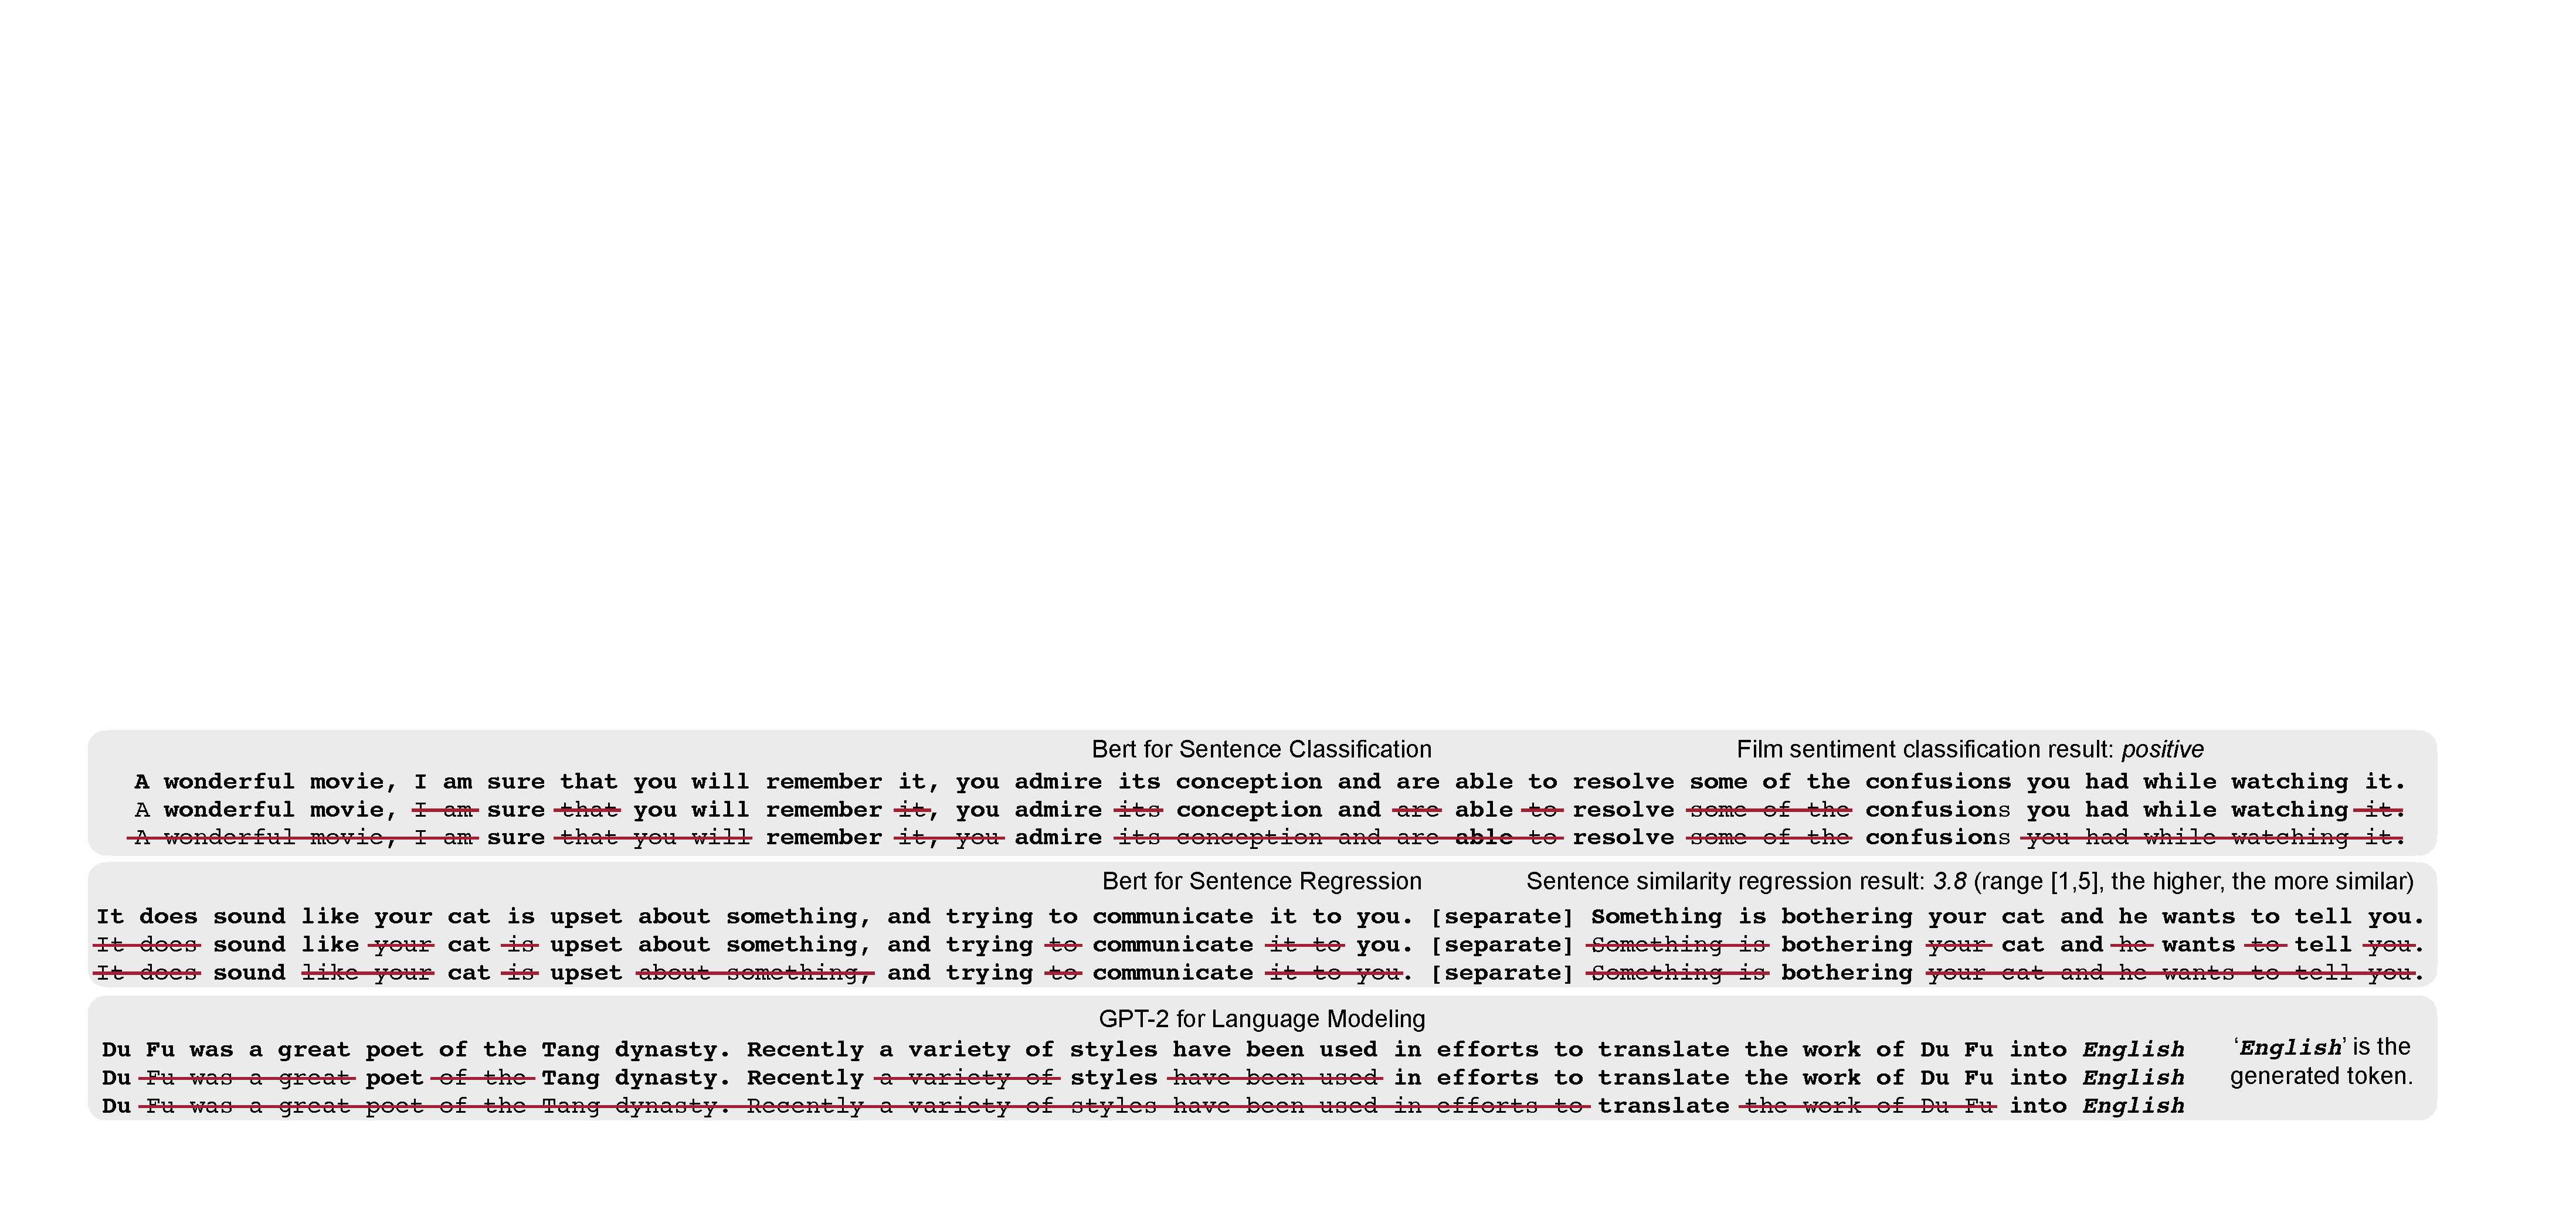
\includegraphics[width=1\textwidth]{figures/pruning_examples.pdf}
    \vspace{-20pt}
    \caption{Examples for cascade token pruning in different models and tasks. \name supports both discriminative models (\bert) and generative models (\gpttwo). Unlike \athree and \mnnfast, cascade token pruning in \name is structured and interpretable.}
    \vspace{-20pt}
    \label{fig:pruning_examples}
\end{figure*}

\begin{figure}[t]
    \centering
    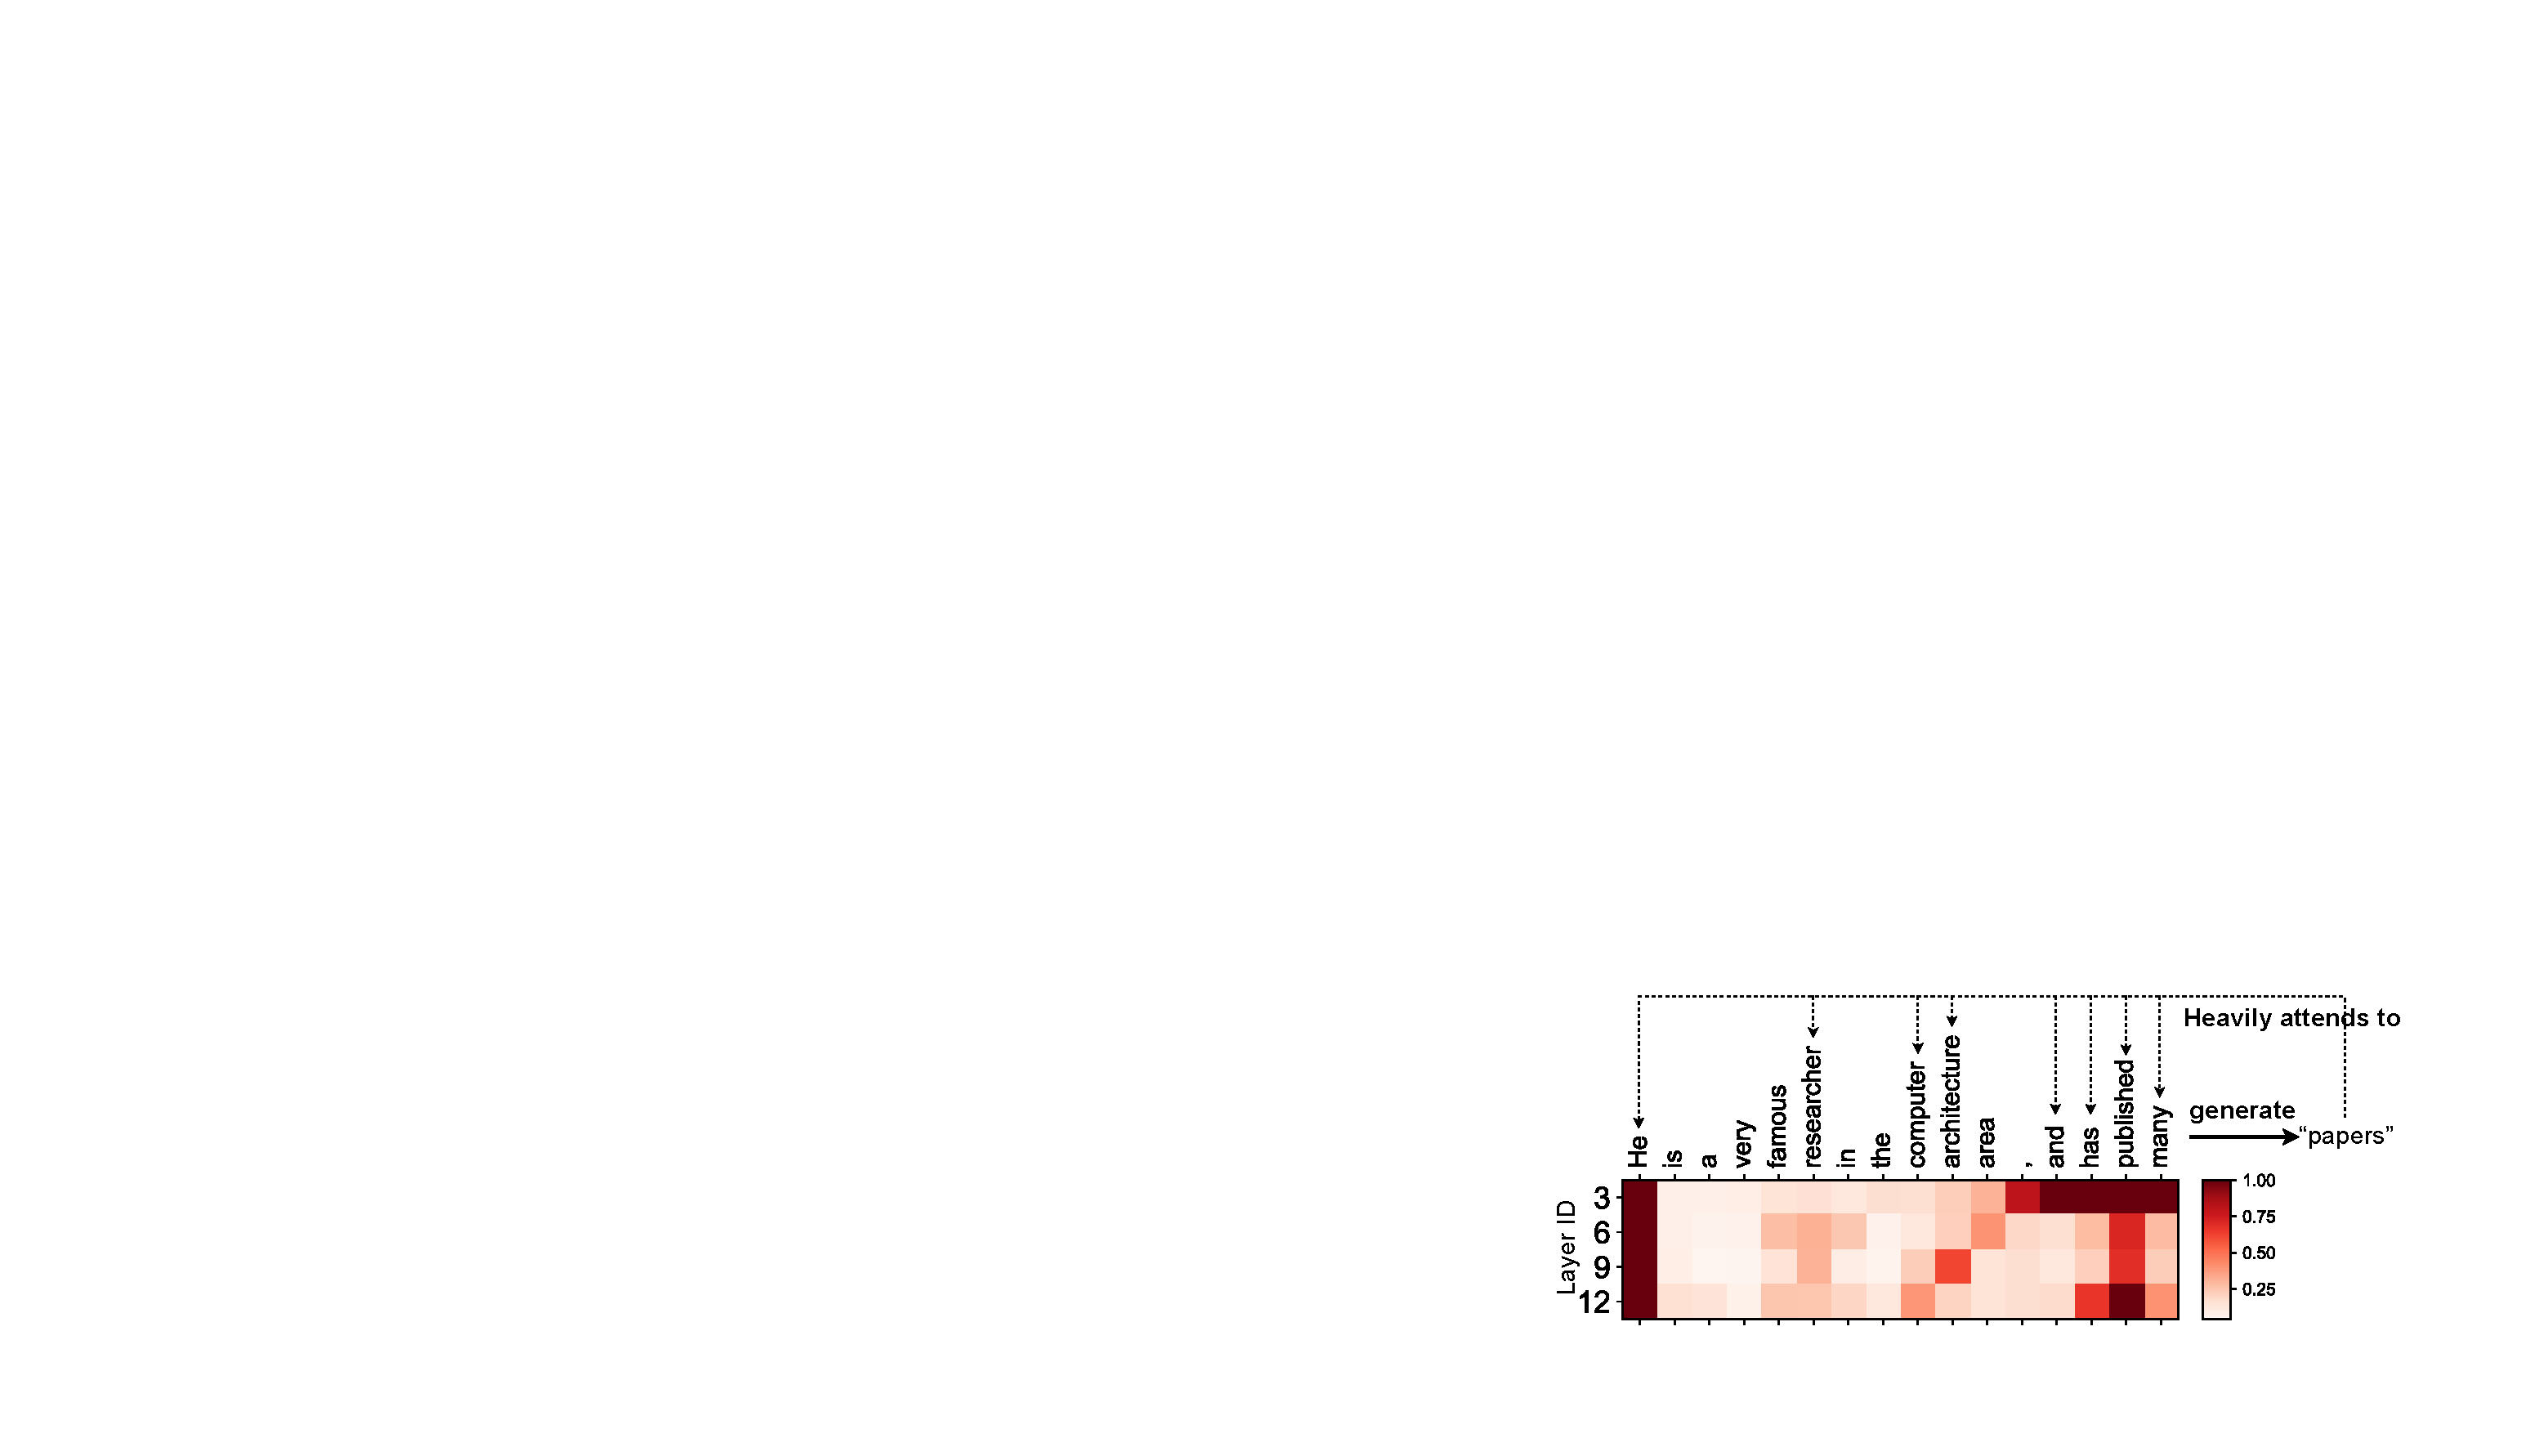
\includegraphics[width=\columnwidth]{figures/heatmap_gpt2.pdf}
    \vspace{-20pt}
    \caption{Cumulative importance scores in \gpttwo. Unimportant tokens are pruned on the fly. Important tokens are heavily attended.
}
\vspace{-15pt}
    \label{fig:heatmap_gpt2}
\end{figure}



